%% +++++++++++++++++++++++++++++++++
%% Setzen von scrreprt
%% +++++++++++++++++++++++++++++++++
\documentclass[
11pt,
titlepage,
a4paper,
abstracton,
twoside,
openright,
chapterprefix,
noappendixprefix,
headsepline,
footsepline,
cleardoubleplain,
bibtotoc,
liststotoc,
pointlessnumbers
]{scrreprt}

%% +++++++++++++++++++++++++++++++++
%% Einbinden von Paketen
%% +++++++++++++++++++++++++++++++++
\usepackage{istitle}
\usepackage{geometry}
\usepackage[utf8]{inputenc} 
\usepackage[T1]{fontenc}
\usepackage{ae,aecompl}
\usepackage{amsmath}
\usepackage{amsthm}
\usepackage{amscd}
\usepackage{amsfonts}
\usepackage{amssymb}
\usepackage{listings}
\usepackage{xcolor}
\usepackage[german,ngerman]{babel}
\usepackage{graphicx}
\usepackage{url}
\usepackage[automark]{scrpage2}
%\usepackage{natbib}
\usepackage{bbm}
\usepackage{array}
\usepackage{booktabs}
\usepackage{threeparttable}
\usepackage{pifont}
\usepackage{placeins}
\usepackage[font=small,labelfont=bf,labelsep=colon]{caption}

% Settings for generating the PDF
% See https://www.tug.org/applications/hyperref/manual.html

\usepackage{hyperref}

\hypersetup{
	pdfinfo={ 
    		Title={Diplomarbeit},
		Creator={TeX},
		Producer={pdfTeX 0.15a},
		Author={},
		CreationDate={D:20091004000000},
		ModDate={D:20130331000000},
		Subject={Master thesis},
		Keywords={}
	},
	pdfpagelayout=TwoColumnRight,
	pdfdisplaydoctitle=true
}



%% Settings for generating the PDF
% See https://www.tug.org/applications/hyperref/manual.html


\hypersetup{
}


 % Links klickbar, vom PDF-Viewer hervorgehoben
%% Settings for generating the PDF
% See https://www.tug.org/applications/hyperref/manual.html


\hypersetup{
	colorlinks, % colored links
	linkcolor=blue,
	filecolor=darkgreen,
	urlcolor=red,
	citecolor=green,
	hypertexnames=false,
}
 % Links klickbar, farbig hervorgehoben
% Settings for generating the PDF
% See https://www.tug.org/applications/hyperref/manual.html


\hypersetup{
	hidelinks=true % for hiding links altogether
}


 % Links klickbar, aber nicht hervorgehoben



%% +++++++++++++++++++++++++++++++++
%% Header
%% +++++++++++++++++++++++++++++++++

% Seitengeometrie
\geometry{a4paper,outer=38mm,inner=26mm,top=40mm,bottom=50mm}

% Definition von arg max
\DeclareMathOperator*{\argmax}{arg\,max}

% Definition von Sternchen
\newcommand{\sig}{\ding{73}}
\newcommand{\ssig}{\ding{72}}

% Definition von Häkchen und Kreuzchen
\newcommand{\h}{\ding{51}}
\newcommand{\x}{\ding{55}}

% Farben definieren
\definecolor{lightgrey}{rgb}{0.99,0.99,0.99}
\definecolor{colKeys}{rgb}{0,0,1}
\definecolor{colIdentifier}{rgb}{0,0,0}
\definecolor{colComments}{rgb}{1,0,0}
\definecolor{colString}{rgb}{0,0.5,0}

\definecolor{darkred}{rgb}{0.5,0,0}
\definecolor{darkgreen}{rgb}{0,0.5,0}
\definecolor{darkblue}{rgb}{0,0,0.5}
\definecolor{green}{rgb}{0,0.7,0}
\definecolor{blue}{rgb}{0,0,0.7}
\definecolor{red}{rgb}{0.7,0,0}
\definecolor{black}{rgb}{0,0,0}

% Quellcode
\lstloadlanguages{XML} 
\lstset{
    float=hbp,
    keywordstyle=\color{colKeys},
    stringstyle=\color{colString},
    commentstyle=\color{colComments},
    basicstyle=\texttt\small,
    identifierstyle=\color{colIdentifier},
    columns=flexible,
    tabsize=2,
    frame=single,
    extendedchars=true,
    showspaces=false,
    showstringspaces=false,
    numbers=none,
    numberstyle=\tiny,
    breaklines=true,
    backgroundcolor=\color{lightgrey},
    breakautoindent=true,
	captionpos=b,
	xleftmargin=\fboxsep,
	xrightmargin=\fboxsep,
	frameround=tttt,
	inputencoding=utf8,
	extendedchars=true,
	literate={ä}{{\"a}}1 {ü}{{\"u}}1 {ö}{{\"o}}1,
}
\lstset{literate= {á}{{\'a}}1 {é}{{\'e}}1 {í}{{\'i}}1 {ó}{{\'o}}1 {ú}{{\'u}}1 {Á}{{\'A}}1 {É}{{\'E}}1 {Í}{{\'I}}1 {Ó}{{\'O}}1 {Ú}{{\'U}}1 {à}{{\`a}}1 {è}{{\`e}}1 {ì}{{\`i}}1 {ò}{{\`o}}1 {ù}{{\`u}}1 {À}{{\`A}}1 {È}{{\'E}}1 {Ì}{{\`I}}1 {Ò}{{\`O}}1 {Ù}{{\`U}}1 {ä}{{\"a}}1 {ë}{{\"e}}1 {ï}{{\"i}}1 {ö}{{\"o}}1 {ü}{{\"u}}1 {Ä}{{\"A}}1 {Ë}{{\"E}}1 {Ï}{{\"I}}1 {Ö}{{\"O}}1 {Ü}{{\"U}}1 {â}{{\^a}}1 {ê}{{\^e}}1 {î}{{\^i}}1 {ô}{{\^o}}1 {û}{{\^u}}1 {Â}{{\^A}}1 {Ê}{{\^E}}1 {Î}{{\^I}}1 {Ô}{{\^O}}1 {Û}{{\^U}}1 {œ}{{\oe}}1 {Œ}{{\OE}}1 {æ}{{\ae}}1 {Æ}{{\AE}}1 {ß}{{\ss}}1 {ű}{{\H{u}}}1 {Ű}{{\H{U}}}1 {ő}{{\H{o}}}1 {Ő}{{\H{O}}}1 {ç}{{\c c}}1 {Ç}{{\c C}}1 {ø}{{\o}}1 {å}{{\r a}}1 {Å}{{\r A}}1 {€}{{\EUR}}1 {£}{{\pounds}}1 }

% Kopf- und Fußzeilen
\pagestyle{scrheadings}
\ihead[]{}
\chead[]{}
\ohead[]{\textsf{\headmark}}
%\ifoot[]{}
%\cfoot[]{}
%\ofoot[]{\textsf{\pagemark}}

% Absätze
\setlength{\parindent}{0pt}
\setlength{\parskip}{2ex}

\def\topfraction{1.0} 
\def\bottomfraction{1.0} 
\def\textfraction{0.0}

\renewcommand*{\partpagestyle}{empty}

% Überschrift des Abstracts
\addto\captionsngerman{\renewcommand*\abstractname{Kurzzusammenfassung}}
% Überschrift des Verzeichnisses der Listings
\addto\captionsngerman{\renewcommand*\lstlistlistingname{Auflistungsverzeichnis}}
% Name von Listings
\addto\captionsngerman{\renewcommand*\lstlistingname{Auflistung}}


%% +++++++++++++++++++++++++++++++++
%% Start des Dokuments
%% +++++++++++++++++++++++++++++++++
\begin{document}

% Titelseite
\title{Extraktion von Entitäten aus Suchergebnissseiten}
\author{Denis Repkov}
\tutor{Professor~Dr.-Ing.~Norbert Fuhr}
{Dipl.-Inform.~Sebastian Dungs}
\thesistype{Masterarbeit}

\logo{Bilder/logo_uni.png}
\timeperiod{Mai 2015}{November 2015}
\pagenumbering{alph}
\maketitle

% Kurzzusammenfassung (Abstract)
\setcounter{page}{2}
\begin{abstract}
\thispagestyle{plain}
Sehr kurze Zusammenfassung der Arbeit
\end{abstract}

% Inhaltsverzeichnis
\pagestyle{scrheadings}
\setcounter{tocdepth}{2}
\tableofcontents

% Text
\cleardoublepage
\pagenumbering{arabic}
\pagestyle{scrheadings}
\sloppy
\chapter{Einleitung}

\section{Motivation}
\label{sec:Motivation}
\paragraph{}
Wenn man im Web nach einem Begriff sucht, kann die Suchanfrage nicht immer sofort genau definiert werden, besonders wenn das Thema der Suche dem Benutzer nicht bekannt ist. Um eine korrekte Anfrage aufzubauen, die die gewünschte Ergebnisse liefert, braucht man mehr Iterationen - mit jeder Iteration wird die Anfrage präzisiert und verbessert. Da moderne Suchmaschinen allerdings keine strukturierte Informationen über die Suchergebnisse, und auf der Suchergebnisseiten vorhandene Entitäten liefern, wird der Benutzer gezwungen, sich jeden gefundenen Dokument manuell anzuschauen, um die Anregungen für neue Suchiterationen zu gewinnen, was als Folge eine niedrige Arbeitsleistung hat.

\paragraph{}
Um den Benutzer bei der Verfeinerung seiner Suchanfragen zu unterstützen, wäre die Erkennung und Extraktion von Entitäten aus der Ergebnissdaten sehr hilfreich. Der Benutzer soll von der Suchmaschine die Ontologien mit den Ergebnisseiten zusammen bekommen, dann kann es anhand der Informationen über extrahierte Entitäten, wie z.B. die Klasse der Entität, ihre Beschreibung und Verlinkungen zu anderen Entitäten, entschieden werden, wie genau die Suchanfrage angepasst werden muss, um erwünschte Daten zu finden.

\paragraph{}
Dabei soll beachtet werden, dass jede natürliche Sprache einen besonderen an dieser Sprache angepassten Verfahren braucht, um erkennen zu können, welche Entitäten in dem Text vorkommen. Für englische Sprache existieren schon jetzt Verfahren und Modellen, mit deren Hilfe die englischsprachige Entitäten extrahiert werden können. Allerdings fällt das Modell für die deutsche Sprache, deswegen findet die Extraktion von deutschsprachigen Entitäten zur Zeit nicht statt.

\paragraph{}
Eine reine Extraktion von Entitäten ist aber nicht ausreichend - der Extraktionschritt sagt nur, welche Tokens in dem Text möglicherweise eine Entität darstellen, die Informationen über die Entität - die dazugehörige Ontologie - fehlt nach dem Extraktionschritt noch. Um die entsprechende Ontologien mit den extrahierten Entitäten verlinken zu können, muss noch EntityLinking durchgeführt werden. Dafür wird für jede extrahierte Entität eine Suche in einer Wissendatenbank durchgeführt. Eine Wissendatenbank ist eine Datenbank, wo Ontologien für diverse Entitäten gespeichert werden. Für die Websuche kann DBpedia als Wissenbasis verwendet werden, allerdings für weniger generische Aufgaben, wie z.B. ein Suchsystem für Ärzte, wo der Suchdomain klar definiert ist, können andere Datenbanken verwendet werden.

\section{Aufgabenstellung}
\label{sec:Aufgabenstellung}
\paragraph{}
Die Arbeit umfasst zwei große Abschnitte: Zuerst soll ein Framework entwickelt werden, der die Extraktion und Verlinkung von Ontologien für deutschsprachige Webseiten ermöglicht. Die Webseiten werden dabei nicht im PlainText ins System eingegeben, sondern als HTML. Deswegen soll der Framework auch rohe Textdaten aus dem HTML extrahieren können. Danach soll ein Proxyserver  entwickelt werden, der die Suchanfragen des Benutzers zuerst an eine herkömmliche Suchmaschine weiterleitet, deren Antwort aber nicht direkt an den Benutzer sendet, sondern an den im ersten Schritt entwickelten Framework, und deren Ausgabedaten (Extrahierte Entitäten mit den verlinkten Ontologien zusammen) an die Suchergebnisse anhängt, und mit den Ontologien angereicherte Ergebnisse an den Benutzer sendet.

Der Extraktionsframework soll auf Basis von Apache Stanbol entwickelt werden, der dem Entwickler eine API für die Manipulation mit Ontologien und für die Anreicherung von Textdaten zur Verfügung stellt. Als Wissendatenbank für die Ontologien soll deutsche Version von DBpedia verwendet werden. Der Proxyserver soll als eine Erweiterung des auf dem Lehrstuhl entwickelten Suchproxys implementiert werden.

\paragraph{}
Die Entwicklung der Stanbol-Erweiterung umfasst folgende Schritte:
\begin{enumerate}
\item Zuerst soll ein Plugin implementiert werden (sogenannter Enhancer), der markiert, welche Tokens möglicherweise einer Entität entsprechen. Dabei wird für jede Mögliche Entität eine grobe Typeinschätzung gemacht (ob das eine Person, eine Organisation, eine geographische Entität oder MISC - eine Entität, die zu keinem anderen Typ passt, ist). Die erkannte Entitäten werden mit bestimmten Annotationen versehen, die für spätere Bearbeitungsschritte benötigt werden. Die Erkennung von Entitäten kann grundsätzlich auf zwei unterschiedliche Art und Weisen implementiert werden:  
\begin{itemize}
\item Es kann ein existierendes Modell für die Erkennung von Entitäten in deutschen Texten benutzt werden (wie Stanford NER).
\item Man kann eigenes Modell mithilfe von OpenNLP trainieren, auf Basis von einem mit Annotationen versehenen Trainingkorpora.
\end{itemize}
Im Rahmen dieser Arbeit sollen beide Methoden implementiert werden.

\item Danach soll die Erweiterung, die die gefundene Entitäten mit passenden Ontologien verlinkt, implementiert werden. Hier können zwei Lösungen eingesetzt werden:
\begin{itemize}
\item Man kann den in Stanbol eingebetteten Plugin verwenden, der den internen Solr-Index verwendet, um die Ontologien mit den entsprechenden Entitäten zu verliken. In diesem Fall muss man einen eigenen Index für deutsche DBpedia aufbauen, und den an den Stanbol anbinden.
\item Man kann auch eine eigene Erweiterung schreiben, die SPARQL-Anfragen verwendet, um die Ontologien aus Online-Version von DBpedia lädt.
\end{itemize}
\end{enumerate}

Die Implementiuerung eines Proxyservers umfasst folgende Schritte:

%\section{Aufbau der Arbeit}
%\label{sec:Aufbau der Arbeit}
\chapter{Grundlagen}
\label{sec:Grundlagen}

\section{Extraktion von Entitäten}
\paragraph{}
%Was sind die Entitäten - kurze Einleitung. Wie genau können die Entitäten aus einem Text extrahiert werden? Welche Einsätze gibt es? Wofür kann man Entitäten verwenden?
Vijay Krishnan hat in seiner Arbeit\cite{Vijay/Vignesh:05} die Extraktion von Entitäten als Suche nach atomaren Elementen im Text und ihre Zuordnung bestimmten vordefinierten Klassen wie Person, Organisation, geographische Lokation usw. definiert. Zum Beispiel betrachten wir folgenden Text aus Wikipedia: ,,Seit dem 1. Januar 2014 ist Bill de Blasio neuer Bürgermeister von New York.``. Dabei soll der Framework, der die Entitäten aus dem Text extrahiert, die Entität \textit{Bill de Blasio} als eine Person erkennen, die Entität \textit{New York} als ein geographisches Objekt, und \textit{1. Januar 2014} als ein Datum.

\lstset{language=java}
\lstinputlisting[captionpos=b,label={lst:ENTITYBEISPIEL},caption={Beispiel einer Entität}]{Listings/entity-beispiel.json}

\paragraph{}
Es stellt sich die Frage, wie genau können die Entitäten für die Benutzerunterstützung bei der Suche eingesetzt werden? Wenn die einzige Information, die dem Benutzer zur Verfügung stehen würde, nur der Name, das Typ und Position der Entität innerhalb des Textes wären, wären Entitäten kaum verwendbar. Aber wenn jeder Entität eine Menge von Eigenschaften (wie Geburtsdatum für eine Person) und Verbindungen zu anderen Entitäten (Z.b. Geburtsort einer Person könnte ein Link auf eine geografische Entität sein) zugeordnet wird, könnte der Benutzer theoretisch die aus der Entität gewonnene Informationen für Präzisierung der Suchanfrage verwendet werden. Ein Beispiel der Entität mit Eigenschaften und Links zu anderen Entitäten findet man in der Auflistung \ref{lst:ENTITYBEISPIEL}.

\paragraph{}
Aber wie genau können die Entitäten aus dem Text extrahiert werden? In dieser Arbeit wird drei verschiedenen Einsätzen zur Extraktion von Entitäten verwendet: Conditional Random Field (CRF) als Teil des Stanford NER Frameworks, Support Vector Machines, implementiert als teil des MITIE-Frameworks und Maximum Entropy based NER, implementiert im OpenNLP Framework.

\subsection{Conditional Random Field}
%Was ist CRF? Wie funktioniert dieser Einsatz? Wo wird er verwendet?
\paragraph{}
CRFs wurden vom Charles Sutton und Andrew McCallum in ihrer Arbeit\cite{Charles/Andrew:10} beschrieben. CRF hilft, die Verteilung $p(y|x)$ mithilfe eines Graph (siehe Abbildung \ref{fig:CRF-Modell}) direkt zu modellieren. Dabei soll jedem Element (Token in unserem Fall) aus dem Eingabevektor $x$ ein entsprechendes Ausgabewert (Label, die die Klasse der Entität beschreibt) aus dem Vektor $y$ zugeordnet werden. CRF basiert auf demselben Basis wie Hidden Markov Models, hat aber den Vorteil, dass die Features nicht als unabhängig betrachtet werden - CRF nimmt an, dass es Abhängigkeiten zwischen Features existieren. Der Nachteil ist, dass CRF langsamer, als HMM ist. Und für die NER sind die Abhängigkeiten zwischen Features schon sehr wichtig - wenn wir z.B. den Satz ,,Ich lese gerade Berliner Zeitung`` analysieren, ohne Abhängigkeiten zwischen Features im Kauf zu nehmen, wird das Wort ,,Berliner`` als Gebäck erkannt, und wenn man die Abhängigkeiten zwischen Nachbarnwörtern betrachtet, erkennt man die Entität ,,Berliner Zeitung``.

\begin{figure}[ht]
\setbox0\vbox{\small}
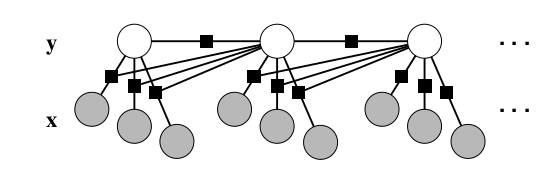
\includegraphics[width=0.7\textwidth]{Bilder/crf-modell-charles-andrew}
\caption{CRF-Modell (die Abbildung ist der Arbeit von Charles Sutton \cite{Charles/Andrew:10} entnommen)}
\label{fig:CRF-Modell}
\end{figure}

\paragraph{}
Die Formel, die die Verteilung $p(y|x)$ beschreibt, lautet 
$$
p(y|x) = \frac{1}{Z(x)}\prod_{t=1}^T\exp \lbrace \sum_{k=1}^K \theta_k f_k(y_t,y_t-1,x_t) \rbrace
$$  

Funktion $f_k$ beschreibt dabei Features, und Vektor $\theta$ - Parameter. Die Funktion $Z(x)$ ist eine Normalisierungsfunktiuon, und wird wie folgt definiert:
$$
Z(x) = \sum_y \prod_{t=1}^T\exp \lbrace \sum_{k=1}^K \theta_k f_k(y_t,y_t-1,x_t) \rbrace
$$
Vektor $x_t$ beinhaltet dabei alle Features, die benötigt werden, um Abhängigkeiten zu berechnen. 

\paragraph{}
Aber wie definiert man Features? Jenny Finkel\cite{Jenny/etal:07} hat folgende Eigenschaften definiert:
\begin{enumerate}
\item Nachbarnwörter: vorheriges Wort, nächstes Wort, alle Wörter innerhalb eines Fensters.
\item Orthographische Eigenschaften.
\item Präfixe und Suffixe.
\item Labelsequenzen.
\end{enumerate}

\subsection{SVM}
\paragraph{}
Support Vector Machines (oder Stützvektormaschine) ist eine Methode zur Klassifizierung von Daten, deren Grundidee\cite{meyer2014support} auf der Abbildung \ref{fig:SVM-INTRO} graphisch dargestellt ist. 

\begin{figure}
\centering
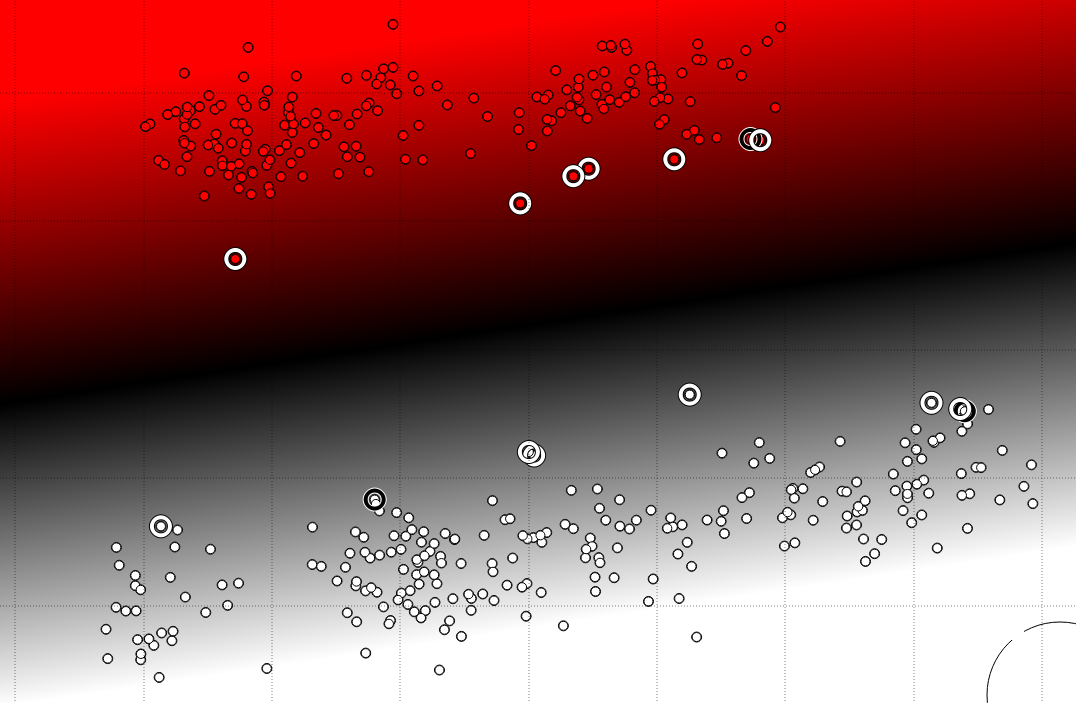
\includegraphics[width=\textwidth,angle=90]{Bilder/svm-intro.png}
\caption{''Die Klassifizierung mithilfe von Stützvektoren''}
\label{fig:SVM-INTRO}
\end{figure}

Der SVM-Klassifikator versucht, für eine Menge von \textbf{linear trennbaren} Punkten in einem Vektorraum eine Hyperebene zu finden, die die Punkte in zwei Klassen aufteilt, und zwar so, dass der Abstand zwischen dieser Trennfläche und den Randpunkten möglichst maximal bleibt.

\paragraph{}
Damit so eine Hyperebene aufgebaut werden könnte, ist es wichtig, dass die Datenpunkte linear trennbar sind. Wenn das SVM-Algorithmus direkt auf nicht linear trennbare Daten angewendet wird, wird die resultierende Trennebene falsch aufgebaut, was auf der Abbildung \ref{fig:SVM-NONLINEAR-ISSUE} zu sehen ist. 

Allerdings sind meiste Daten, mit denen man in der realen Welt arbeiten muss, nicht linear trennbar, und damit kann das SVM-Algorithmus nicht in seiner ursprünglichen Form verwendet werden. Allerdings gibt es eine Möglichkeit, mit einer Erweiterung von SVM-Einsatz auch nicht linear trennbare Daten zu klassifizieren. Dazu muss das ursprüngliche Eigenschaftensraum auf ein Raum höherer Dimension abgebildet werden, und zwar so, dass die Datenpunkte in neuem Raum linear trennbar wären\cite{Hearst:98}.

Das Verfahren, das solche Abbildung ermöglicht, heißt ,,Kernel``, und ist in der Arbeit von Hsu\cite{hsu2003practical} beschrieben. Ein Kern ist eine Funktion 
$K(x_i,x_j) = \phi(x_i)^T \phi(x_j)$, die den Punkt im ursprünglichen Raum $R^{n_1}$ auf ein Punkt im Raum $R^{n_2}$ abbildet, so dass $n_1 < n_2$ ist. In der Praxis sind laut Hsu\cite{hsu2003practical} folgende Kernfunktionen etabliert:
\begin{enumerate}
\item Lineares Kern: $K(x_i,x_j) = x_i^T x_j$
\item Polynominales Kern: $K(x_i,x_j) = (\gamma x_i^T x_j + r)^d, \gamma > 0$
\item Radiale Basisfunktion (RBF): $K(x_i,x_j) = exp(-\gamma \Vert x_i - x_j \Vert^2), \gamma > 0$
\item Sigmoid : $K(x_i,x_j) = tanh(\gamma x_i^T x_j + r)$
\end{enumerate}
Die Variablen $\gamma$, $r$ und $d$ sind benutzerdefinierte Kernelparameter.

\begin{figure}
\centering
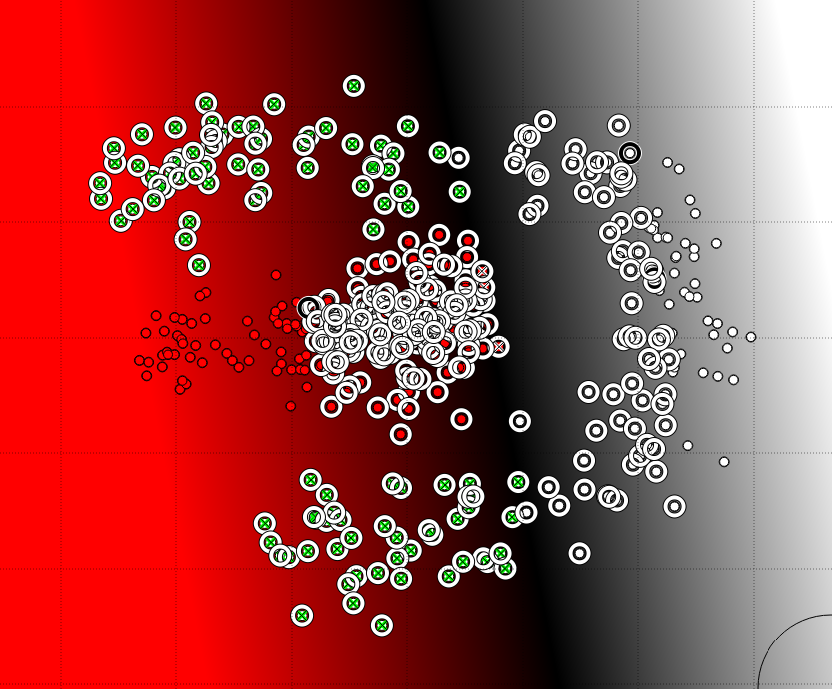
\includegraphics[width=\textwidth,angle=90]{Bilder/svm-nonlinear-issue.png}
\caption{''SVM Algorithmus angewandt auf nicht linear trennbare Daten''}
\label{fig:SVM-NONLINEAR-ISSUE}
\end{figure}

\begin{figure}
\centering
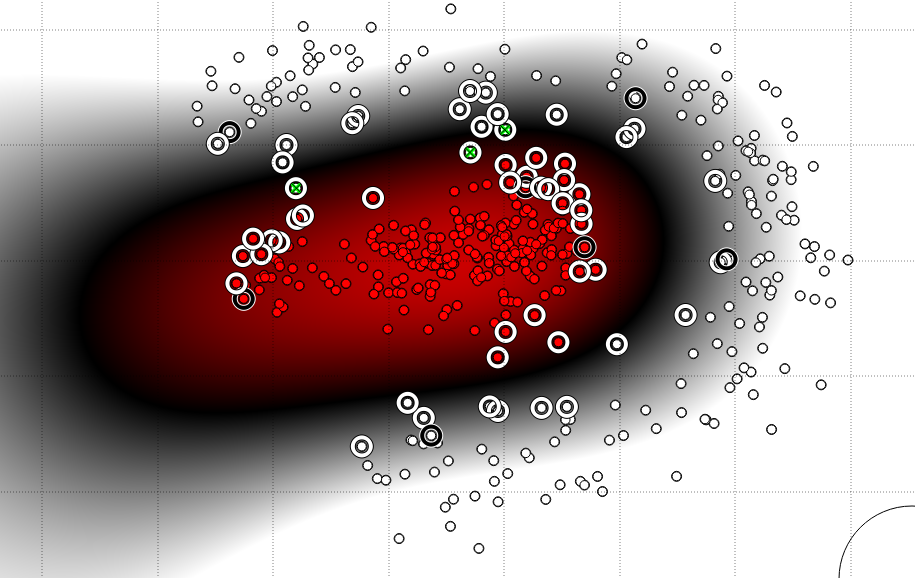
\includegraphics[width=\textwidth,angle=90]{Bilder/svm-nonlinear-rbf.png}
\caption{''SVM-Algorithmus mit einem RBF-Kern angewandt auf nicht linear trennbare Daten''}
\label{fig:SVM-NONLINEAR-ISSUE}
\end{figure}

\paragraph{}
%Und wie kann man SVMs in NEr einsetzen?
Der Einsatz von Stützvektoren für Extraktion von Entitäten ist in der Arbeit von Kazama\cite{kazama2002tuning} beschrieben. Obwohl es in dieser Arbeit um Extraktion von Entitäten aus englischsprachigen medizinischen Texten geht, kann dasselbe Prinzip auch auf deutsche Texte angewendet werden, wenn man das richtige Korpus für Training zur Verfügung stellt. Um SVMs für Extraktion von Entitäten einsetzen zu können, muss noch eine Erweiterung zum ursprünglichen Algorithmus gemacht werden, zusätzlich zum Kerneleinsatz - Stützvektoren können generell zwischen zwei Klassen von Objekten unterscheiden (ein Stützvektoreinsatz kann sagen, ob das Objekt der Klasse $C_a$ oder der Klasse $C_b$ gehört), und bei Entitäten gibt es mehr als zwei Klassen. Um diese Beschränkung umzugehen, wird SVM-Algorithmus auf eine der folgenden Arten und Weisen erweitert:

\begin{itemize}
\item Für jede mögliche Entitätsklasse wird ein SVM aufgebaut, der entscheidet, ob das Token der Klasse $C_a$ oder dem Rest der Klassen gehört.
\item Für jede Paar $(C_a, C_b)$ von möglichen Entitätstypen wird ein SVM erzeugt, der feststellen muss, ob das Wort den Typ $C_a$ oder $C_b$ hat. Die Klasse, die von der Mehrheit von SVMs gewählt wurde, gewinnt.
\end{itemize}

\paragraph{}
Vorteile von SVM-Einsatz anderen Methoden gegenüber:
\begin{itemize}
\item A
\end{itemize}

Nachteile von SVMs anderen Einsätzen gegenüber:
\begin{itemize}
\item B
\end{itemize}

\subsection{Maximum Entropy based NER}
%Was ist ME NER? Wo wird er verwendet? Welche Vor- und Nachteile hat dieser Einsatz im Vergleich zum CRF?
\paragraph{}
Dieses Framework wurde in der Arbeit von Andrew Borthwick\cite{Andrew:99} vorgestellt. In diesem Modell wird auch wie im CRF mit der Wahrscheinlichkeit $p(y|x)$ gearbeitet, allerdings ist ME NER kein graphisches Framework. Die Formell, die die Verteilung für ME-Modell beschreibt, sieht wie folgt aus:
$$
P(y|x) = \frac{1}{Z(x)}\prod_i \alpha_i^{g_i(x,y)}
$$
$g_i$ ist eine binäre Funktion, die eine bestimmte Feature beschreibt, und $\alpha_i$ ist das Parameter, der mit der Eigenschaft assoziiert wird. $Z(x)$ ist eine Normalisierungsfunktion, die wie folgt aussieht:
$$
Z(x) = \sum_y \prod_i \alpha_i^{g_i(x,y)}
$$
Eigenschaften $g_i$ können in zwei Klassen geteilt werden: lokale und globale Features. Hai und Hwee\cite{Hai/Hwee:02} definieren unter anderem folgende Eigenschaften, die auch im OpenNLP-Framework eingesetzt werden:
\begin{enumerate}
\item Globale Eigenschaften:
\begin{enumerate}
\item Personenpräfixe für bestimmtes Wort in anderen Sätzen des Dokumentes: z.B. wenn wir im Text zuerst die Tokens ,,Frau Sony`` treffen, und dann einfach ,,Sony``, dann soll angenommen werden, dass ,,Sony`` eine Entität mit dem Typ ,,Person`` ist.
\item Abkürzungen: wenn in einem Satz mehr Wörter nacheinander groß geschrieben werden, wie z.B. ,,Deutsche Demokratische Republik``, dann wird in dem Text nach entsprechender Abkürzung gesucht: ,,DDR``, und wenn Abkürzung eine Entität ist, können auch alle entsprechende Tokens als eine Entität markiert werden.
\end{enumerate}
\item Lokale Eigenschaften:
\begin{enumerate}
\item Ob das Wort großgeschrieben wird.
\item Ob vorheriges oder nächstes Wort großgeschrieben wird.
\item Ob alle Zeichen im Token großgeschrieben werden.
\item Ob es ein Punkt am Ende des Wortes steht.
\item Ob der Token Zahlen beinhaltet, und falls ja, wie viel.
\item Ob das Wort das Prozent- oder Dollarzeichen beinhaltet.
\item Suffixe und Präfixe (wie ,,Frau`` oder ,,GmbH``).
\end{enumerate}
\end{enumerate}


\section{Wissendatenbanke}
%Was sind Wissendatenbanke? Wieso brauchen wir die in unserer Arbeit? Wie sucht man nach Entitäten in einer Wissendatenbank? Kurze Einleitung in SPARQL+RDF.
\paragraph{}
Um die extrahierte Entitäten mit Ontologien anzureichern, braucht man selbstverständlich eine Datenbank, wo alle Informationen zu den Entitäten gespeichert werden. Solche Datenbanken nennt man ,,Wissendatenbanken``. Solche Datenbanke sind keine herkömmliche relationale Datenbanke, da man die Ontologien mit ihrer hierarchischen Struktur zwar auf ein relationales Modell abbilden lassen kann, aber es gibt bessere Datenstrukturen und Anfragesprachen, die die Arbeit mit Ontologien für die Entwickler einfacher machen.

\paragraph{}
Zur Beschreibung von Ontologien dient das RDF-Format\footnote{\url{http://www.w3.org/2001/sw/wiki/RDF}}. Dieses Format basiert auf XML, und gibt dem Entwickler eine einfache Möglichkeit, Hierarchische Daten zu beschrieben. Die Ontologie im RDF-Format kann z.B. wie folgt aussehen:
\lstset{language=XML}
\lstinputlisting[captionpos=b,label={lst:RDFBEISPIEL},caption={Beispiel einer Ontologie im RDF-Format}]{Listings/examplerdf.xml}

\paragraph{}
Als Anfragesprache für RDF wird SPARQL\footnote{\url{http://www.w3.org/2001/sw/wiki/SPARQL}} eingesetzt. Diese Sprache sieht SQL ähnlich aus, operiert allerdings nicht auf relationalen Daten, sondern auf RDF-Graphen. 

Zum Beispiel, wenn die Fläche der Stadt Duisburg und das Bundesland, wo die Stadt liegt, gebraucht werden, kann die SPARQL-Anfrage wie folgt aussehen:
\lstset{language=SPARQL}
\lstinputlisting[captionpos=b,label={lst:SPARQLBEISPIEL},caption={Beispiel einer SPARQL-Anfrage}]{Listings/sparqlexample.sql}

Die Antwort wird dann im Form eines RDF-Datensatzes geliefert:
\lstset{language=XML}
\lstinputlisting[captionpos=b,label={lst:SPARQLRESULT},caption={Beispiel der Antwort auf eine SPARQL-Anfrage}]{Listings/sparqlresult.xml}
%\chapter{Verwandte Arbeiten}

\section{Arbeiten zum Thema A}

In einer vielzitierten Arbeit stellten \cite{Abecker/etal:00} das KnowMore-Projekt dar.

Außerdem wurde noch das KnowMore-Projekt \citep{Abecker/etal:00} in die Untersuchung einbezogen.

Außerdem wurde noch das KnowMore-Projekt \citep*{Abecker/etal:00} in die Untersuchung einbezogen.


In einer vielzitierten Arbeit stellten \citet{Abecker/etal:00} das KnowMore-Projekt dar.

In einer vielzitierten Arbeit stellten \citet*{Abecker/etal:00} das KnowMore-Projekt dar.

Das KnowMore-Projekt wurde bereits im Jahr \citeyear{Abecker/etal:00} von \citeauthor{Abecker/etal:00} vorgestellt.

Das KnowMore-Projekt wurde bereits im Jahr \citeyear{Abecker/etal:00} von \citeauthor*{Abecker/etal:00} vorgestellt.




%\chapter{Das Konzept}
\label{sec:Das Konzept}

\chapter{Grundlegende Ideen}
Hier werden die grundlegenden Ideen des eigenen Kozept beschrieben.


\chapter{Implementierung}
\label{sec:Implementierung}

\section{Einleitung}
Um eine richtige Architektur des Systems auswählen zu können, fassen wir kurz die benötigte Komponenten zusammen:
\begin{itemize}
\item Eine Komponente für Training eines NER-Modells.
\item Eine Komponente für Extraktion von Entitäten aus deutschsprachigen Texten.
\item Ein Filter für ,,unpassende`` Entitäten, der alle Entitäten, die bestimmte Kriterien nicht erfüllen, herausfiltert.
\item Eine Komponente für Verlinkung von extrahierten Entitäten mit den Eigenschaften aus einer Wissensdatenbank.
\item Eine API für Anreicherung von Suchergebnissen.
\end{itemize}

Damit alle aufgelistete Anforderungen im Rahmen dieser Arbeit implementiert werden könnten, muss ein Framework verwendet werden, das eine API für die Arbeit mit semantischen Daten ermöglicht, und folgende Voraussetzungen erfüllt:
\begin{enumerate}
\item Quelltexte des Frameworks müssen frei verfügbar sein, damit die entsprechende Erweiterung implementiert werden könnte.
\item Das Framework muss dem Entwickler die Möglichkeit geben, mehrere Algorithmen für Extraktion von Entitäten gleichzeitig einzusetzen, damit alle im Kapitel ,,Grundlagen`` beschriebene Algorithmen implementiert werden könnten.
\item Das Framework soll dem Entwickler eine REST-API zur Verfügung stellen, mit deren Hilfe auf Funktionen des Systems zugegriffen werden könnte, damit eine Integration mit Drittapplikationen (Siehe Sektion \ref{sec:Problemstellung}) implementiert werden könnte. Die zur Verfügung gestellte REST-API kann dabei von der Anreicherung-API direkt verwendet werden.
\end{enumerate}

Im Rahmen dieser Arbeit wurde als solches Framework Apache Stanbol\footnote{\url{http://stanbol.apache.org/} (Zuletzt abgerufen am 04. November)} ausgewählt. Obwohl es andere Systeme, wie Alchemy API \footnote{\url{http://www.alchemyapi.com/}} gibt, die auch deutsche Sprache unterstützen, hat Stanbol gravierende Vorteile anderen Frameworks gegenüber:
\begin{itemize}
\item Die Quelltexte von Stanbol sind frei verfügbar, was die Entwicklung einer Erweiterung einfacher macht. Im Gegenteil dazu ist Alchemy API ein ,,Black Box`` - es gibt keine Möglichkeit, sich die in diesem Framework verwendete Algorithmen anzugucken oder die zu ändern, es gibt keine Möglichkeit, eigene Anpassungen durchzuführen.
\item Stanbol stellt dem Entwickler eine eingebettete REST-API zur Verfügung, was eine Ankopplung an Drittsysteme erleichtert.
\item Stanbol hat eine modulare Architektur, was bedeutet, dass die in dieser Arbeit benötigte Komponente sich genau so implementieren lassen, wie die beschrieben wurden, als voneinander getrennte Module.
\item Außerdem wird dem Entwickler eine interne Wissensdatenbank zur Verfügung gestellt, was die Benutzung einer getrennter Software für die Implementierung der Verlinkung unnötig macht. 
\end{itemize}
Durch die beschriebene Vorteile erfüllt Apache Stanbol alle im letzten Paragraph erwähnte Bedingungen.

\section{Apache stanbol}
Apache Stanbol stellt dem Entwickler eine Plugin-API zur Verfügung, mit deren Hilfe neue Features wie Extraktion von Entitäten aus deutschen Texten leicht implementiert werden können. Die Liste von verfügbaren Modulen ist auf der Abbildung \ref{fig:komponenten} zusammengefasst.

\begin{figure}[ht]
\centering
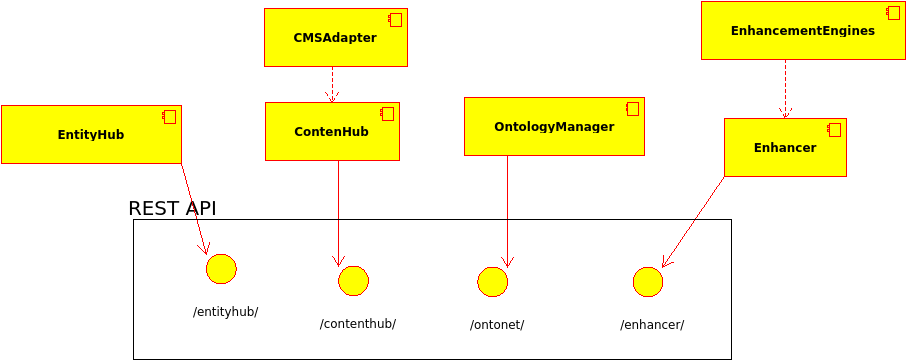
\includegraphics[width=0.6\textwidth]{Bilder/komponenten.png}
\caption{''Komponentendiagramm vom Stanbol''}
\label{fig:komponenten}
\end{figure}

\begin{itemize}
\item \textbf{EntityHub} ist die interne Datenbank, wo die Informationen über Entitäten gespeichert werden. Diese kann sowohl mithilfe von Java API als auch über eine REST-Schnittstelle für die Verlinkung benutzt werden. Als Datenquelle können sowohl ,,Referenced Sites`` (externe Datenquellen die sich auf anderen Maschinen befinden, und auf die EntityHub per Netzwerk zugreift) als auch lokale Indexes verwendet werden. Man kann EntityHub als eine Art von Aggregator betrachten, der mehrere Wissensdatenbanken über eine einheitliche API zur Verfügung stellt. 
\item \textbf{Enhancer} und \textbf{EnhancementEngine} sind die Kernkomponenten von Stanbol, die für die Anreicherung von Texten mit Annotationen zuständig sind.
\item \textbf{OntologyManager} wird, wie sagt der Name, für die Verwaltung von Ontologien zuständig.
\item \textbf{ContentHub} wird für die Integration mit CMS gebraucht und stellt eine Datenbank für das \textit{Content} einer CMS zur Verfügung (nicht für die Entitäten!).
\end{itemize}
Im Rahmen dieser Arbeit werden nur Engines und EntityHub gebraucht, andere Module sind für die Extraktion von Entitäten irrelevant.

\paragraph{}
Die grundlegende Idee, die die Architektur von Stanbol prägt, heißt ,,Pipelining`` - ein Fließband, das mehrere Textverarbeitungsschritte miteinander verknüpft, und eine flexible Konfiguration von Contentanreicherung ermöglicht. Jedes Element dieses Fließbandes wird ,,Engine`` genannt. Von dem Blickwinkel der Architektur wird jedes Engine als eine selbstständige Blackbox implementiert, die am Eingang den Text, der angereichert werden soll, mit den von anderen Engines hinzugefügten Annotationen zusammen, bekommt, und am Ausgang neue Annotationen liefert. 

Die Engines werden in sogenannte Ketten zusammengebunden - der Ausgang von einem Engine wird mit dem Eingang von einem anderen Engine verbunden, und so wird eine virtuelle Kette aufgebaut. Das erste Element in dieser Kette bekommt dabei als Eingang den Text eines mithilfe von einer Suchmaschine gefundenen Snippets, und der Ausgang von dem letzten Element wird zu dem Benutzer geschickt.

Auf der Abbildung \ref{fig:ENGINEPIPELINE} wird der Aufbau der in dieser Arbeit verwendeter Engine-Kette noch einmal grafisch dargestellt.
\begin{figure}[ht]
\centering
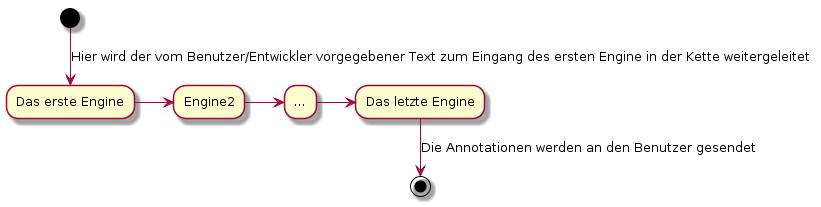
\includegraphics[width=\textwidth]{Bilder/enchancer.png}
\caption{''Graphische Darstellung des Anreicherungspipelines''}
\label{fig:ENGINEPIPELINE}
\end{figure}
Nachdem der Text, der angereichert werden soll, über REST API ausgelesen wurde, werden zuerst rohe Textdaten aus HTML extrahiert, was für Anreicherung von Webseiten notwendig ist. Falls die Daten aber schon im Plaintext gesendet wurden, wird dieser Schritt ignoriert. Danach muss die Sprache des Textes erkannt werden, anhand deren entschieden wird, ob der Text angereichert werden kann. Für die Erkennung der Sprache stellt Stanbol bereits ein Engine \footnote{\url{https://stanbol.apache.org/docs/trunk/components/enhancer/engines/langidengine.html} (zuletzt abgerufen am 10. November)} zur Verfügung.

Falls die Sprache von der Kette unterstützt wird, werden die Sätze und Tokens extrahiert. Die Engines für die Erkennung von Sätzen und Tokens, die deutsche Sprache unterstützen, sind als Standardteil der API verfügbar.

Anschließend können aus dem Text, der vorverarbeitet wurde, Entitäten extrahiert werden. Nach den Extraktion-, Verlinkung- und Filterungsschritten wird der mit Annotationen angereicherte Text über eine REST-Schnittstelle zurückgegeben.

Als Entwickler muss man aber gleich beachten, dass die interne Implementierung von Ketten diese Architektur leider nicht anschaulich abbildet. Wie es auf der Abbildung \ref{fig:REALPIPELINE} zu sehen ist, gibt es intern keine Pipeline - stattdessen wird es für jeden Text, der angereichert werden soll, eine Instanz der Data-Klasse ,,ContentItem`` erzeugt, die zwischen allen Engines der Kette geteilt wird. Die Implementierung eines Engines hat technisch gesehen weder Ein- noch Ausgang, und benutzt stattdessen eine Instanz von ,,ContentItem``, um die Informationen mit anderen Engines auszutauschen. Die Reihenfolge von Elementen in der Engine-Kette bestimmt deswegen nicht, wie die Ein- und Ausgänge von Engines miteinander verbunden werden sollen, sondern die Reihenfolge, in der die Engines ausgeführt werden müssen.

\begin{figure}[ht]
\centering
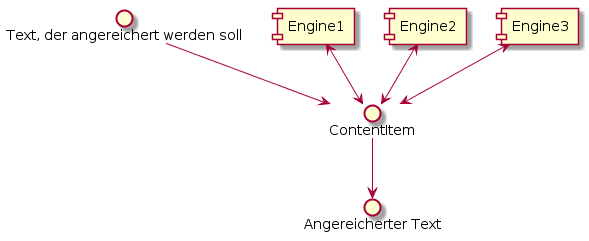
\includegraphics[width=\textwidth]{Bilder/realarch.png}
\caption{''Interne Implementierung einer Engine-Kette''}
\label{fig:REALPIPELINE}
\end{figure}
Der Nachteil solcher Architektur ist, dass mehrere Engines unter Umständen auf dieselbe Instanz von ,,ContentItem`` \textbf{gleichzeitig} zugreifen können, was bei Schreibzugriffen zur Beschädigung von Daten führen kann. Deswegen soll jedes Engine die Instanz von ,,ContentItem`` während des Schreibzugriffs sperren lassen.

Der Vorteil dieser Architektur besteht darin, dass bei Bedarf mehrere Engines parallel für den gleichen Content ausgeführt werden können. Dies kann z. B. dann nützlich sein, wenn es in mehreren Wissensdatenbanken gleichzeitig nach den Informationen über eine Entität gesucht werden muss. Da das ,,ContentItem``-Objekt nur dann mit einem Lock gesperrt werden muss, wenn die Daten \textbf{geschrieben} werden, könnte \textbf{die Suche} in mehreren Wissensdatenbanken parallel durchgeführt werden.

Um sicherstellen zu können, dass nur die Engines, die eine parallele Ausführung unterstützen, parallel gestartet werden, muss der Entwickler in der Konfiguration des Engines explizit eingeben, ob eine parallele Ausführung für das entwickelte Engine möglich ist.

\section{Extraktion von Entitäten} \label{sec:extraktimpl}
Da die Vorverarbeitungsschritte bereits als Teil von Stanbol implementiert sind, ist die Erkennung von Entitäten das erste Modul, das entwickelt werden muss. Die Schritte, die für die Entwicklung eines Engines unternommen werden müssen, lassen sich wie folgt definieren:
\begin{itemize}
\item Ein Engine wird als ein Objekt der Klasse ,,AbstractEnhancementEngine`` implementiert. 
\item Diese Klasse soll dem Framework folgende Methoden zur Verfügung stellen, die die Integration des Engines in eine Enginekette ermöglichen:
\begin{itemize}
\item Eine Aktivierungsmethode, die ein mal beim Start des Engines aufgerufen wird. Diese Methode soll das für das Engine benötigte Modell aus einer Datei laden (ein vortrainiertes SVM-Modell, z. B.).
\item Die Methode, die für den angegebenen Text sagt, ob das Engine diesen Text anreichern kann. Dadurch wird sichergestellt, dass nur die Sprache, die Engine tatsächlich unterstützt, bearbeitet wird.
\item Die Hauptmethode, die für den angegebenen Text Annotationen berechnet.
\end{itemize}
\item Die Ketten, die Engines miteinander verbinden, können sowohl während der Laufzeit als auch vor dem Kompilieren des Systems in einer Konfigurationsdatei definiert werden.
\end{itemize}

\subsection{StanfordNER} \label{subsec:stanfordner}
\paragraph{}
Die erste Anreicherungskette wurde auf Basis von StanfordNER\cite{Jenny/etal:07} aufgebaut. Dieses Framework implementiert das CRF-Algorithmus und stellt ein Modell für die deutsche Sprache zur Verfügung\cite{faruqui10:_training}. Der Nachteil dieses Engines ist, dass es nur ein vortrainiertes Modell zur Verfügung gestellt wird - die Korpora selbst, auf deren Basis ein eigenes Modell trainiert werden könnte, stehen nicht zur Verfügung. Der Vorteil dabei ist, dass es insgesamt zwei vortrainierte Modelle zur Verfügung stehen:

\begin{enumerate}
\item HGC - Huge German Corpus-generalized classifier - dieses Modell wurde auf Texten aus Zeitungen trainiert.
\item deWac - dieser Klassifikator wurde auf Texten aus Internet trainiert.
\end{enumerate}

Dieses Framework stellt außerdem die Möglichkeit zur Verknüpfung von mehreren Modellen miteinander zur Verfügung. Deswegen kann es im Rahmen dieser Arbeit neben dem Austesten von oben genannten Modellen auch ein kombiniertes Modell getestet werden - es ist möglich, dass ein kombiniertes Modell mehr Entitäten im Text finden könnte, andererseits steigt dabei die Wahrscheinlichkeit von False-Positive-Antworten.

Dieses Framework ist auch für die Vorverarbeitung - Zerlegung des Textes in einzelne Sätze und Zerlegung von Sätzen in einzelne Tokens - verantwortlich. Deswegen sind für den auf Stanford-NER basierten Ansatz nur zwei Vorverarbeitung-Engines notwendig:
\begin{enumerate}
\item Tika-Engine für die Extraktion von rohen Textdaten aus HTML.
\item Spracherkennungsmodul, mit deren Hilfe sichergestellt wird, dass die Analyse nur für deutsche Sprache gestartet wird.
\end{enumerate}

Das Klassendiagramm für dieses Engine ist auf der Abbildung \ref{fig:stanfclasses} zu sehen.

\begin{figure}[ht]
\centering
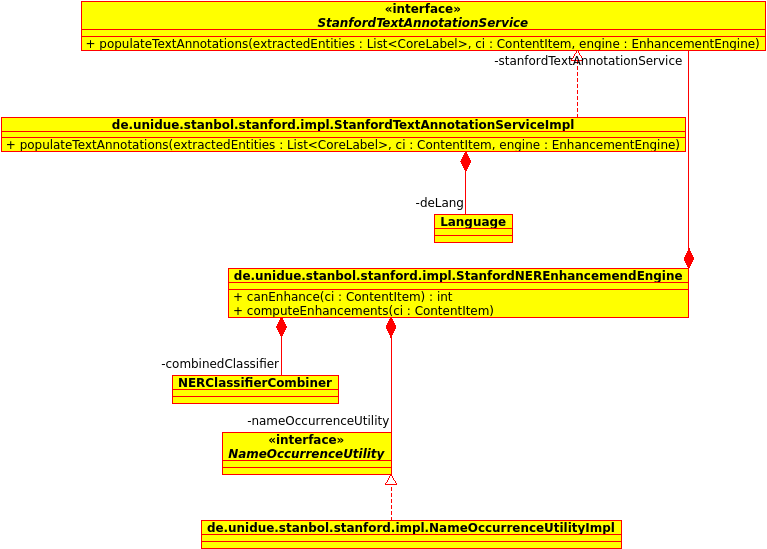
\includegraphics[width=\textwidth]{Bilder/stanford-classes.png}
\caption{''Klassendiagramm  des Stanford-Engines''}
\label{fig:stanfclasses}
\end{figure}
\begin{itemize}
\item Die Klasse \textit{StanfordNEREnhancementEngine} ist die Hauptklasse, die nach den Entitäten im Text sucht.
\item \textit{NERClassifierCombiner} ist die interne Klasse des StanfordNER-Frameworks und stellt die Schnittstelle zum Kombinieren von mehreren NER-Modellen zur Verfügung.
\item \textit{NameOccurenceUtility} ist eine Hilfsklasse, die die Daten zwischen StanfordNER- und Stanbol-Format umwandelt.
\item \textit{StanfordTextAnnotationService} ist ein Hilfsservice, das die vom Engine gefundene Entitäten zum ,,ContentItem`` als Annotationen hinzufügt.
\end{itemize}

\subsection{OpenNLP}
%Beschreibung des OpenNLP-Einsatzes.
Das weitere Algorithmus, das im Rahmen dieser Arbeit verwendet wurde, ist MaximumEntropy. Es wurde als Teil der OpenNLP\footnote{\url{http://opennlp.apache.org/} (Zuletzt abgerufen am 30. Oktober)}-API implementiert. OpenNLP ist ein quelltextoffenes Framework für maschinelle Sprachverarbeitung. Das Framework ist genau wie Stanbol modular aufgebaut, und stellt folgende Funktionalität zur Verfügung:

\begin{itemize}
\item Erkennung von Sätzen. Genau wie für die Extraktion von Entitäten wird für die Satzerkennung ein Maximum-Entropy-Modell verwendet, das vorher trainiert werden muss. Ein Modell für die deutsche Sprache, trainiert auf der Basis von TIGER-Korpus, das in nachfolgendem Kapitel beschrieben ist, ist bereits als Teil des Frameworkes verfügbar.
\item Zerlegung von Sätzen in Tokens, die auf zwei Arten und Weisen durchgeführt werden kann:
\begin{itemize}
\item Die Zerlegung kann ohne vortrainiertes Modell, nur anhand von den in dem Text vorhandenen Leerzeichen, erfolgen.
\item Es kann ein ME-Modell verwendet werden, um Tokens zu erkennen. Der Nachteil dieser Methode ist, dass das Modell zuerst trainiert werden muss, wozu ein Korpus gebraucht wird. Da ein Modell für die Tokenisierung von deutschen Texten als Teil des OpenNLP-Frameworks verfügbar ist, wird im Rahmen dieser Arbeit die modellbasierte Methode verwendet.
\end{itemize}
\item POS-Tagging - die Erkennung und Annotierung von Wortarten - während dieses Vorgangs wird jedem Token eine entsprechende Wortart zugeordnet.
\item Erkennung von Entitäten mithilfe von einem vortrainierten ME-Modell. Hierfür stellt OpenNLP kein vortrainiertes Modell für die deutsche Sprache zur Verfügung.
\end{itemize}

Der Vorteil dieses Engines ist, dass es als Teil vom Stanbol dem Entwickler zur Verfügung steht, und muss deswegen nicht manuell integriert werden. Allerdings müssen die entsprechende ME-Modelle für die Extraktion von deutschsprachigen Entitäten vom Entwickler trainiert werden, worauf in der Sektion \ref{subsec:decor} angegangen wird.

Das Klassendiagramm für das OpenNLP-Engine ist auf der Abbildung \ref{fig:onlpuml} definiert. Es werden insgesamt nur drei Klassen verwendet:
\begin{itemize}
\item Die Basisklasse \textit{NEREngineCore}, die die Extraktion von Entitäten mithilfe vom ME-Algorithmus implementiert.
\item Die Klasse \textit{CustomNERModelEnhancementEngine}, die von der Basisklasse erbt, und für Behandlung von benutzerdefinierten Modellen zuständig ist.
\item Die Konfigurationsklasse \textit{NEREngineConfig}.
\end{itemize}

\begin{figure}[ht]
\centering
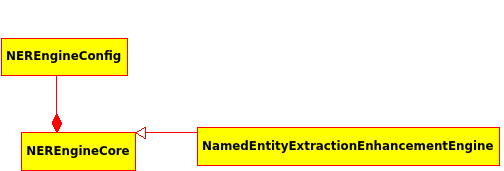
\includegraphics[width=\textwidth]{Bilder/onlp-classes.png}
\caption{''Klassendiagramm  des OpenNLP-Engines''}
\label{fig:onlpuml}
\end{figure}

\subsection{MITIE}
\paragraph{}
Der Einsatz, das implementiert werden soll, ist SVM-Algorithmus. Als Basis wurde für diese Arbeit MITIE\footnote{\url{https://github.com/mit-nlp/MITIE}}-Framework ausgewählt. MITIE steht für ,,MIT Information Extraction`` - ein Framework zur Extraktion von Entitäten und zur Erkennung von binären Relationen. Wie erwähnt, verwendet dieses Framework SVM als Basisalgorithmus für Erkennung von Entitäten, und soll deswegen auch bessere Ergebnisse als OpenNLP oder StanfordNER zeigen können.

\paragraph{Vor- und Nachteile}
\begin{itemize}
\item Vorteile des MITIE-Einsatzes:
\begin{enumerate}
\item Höhere Qualität der Extraktion, im Vergleich zu Maximum Entropy oder CRF.
\item Die Geschwindigkeit der Extraktion ist nicht viel kleiner, als die bei anderen Einsätzen.
\end{enumerate}
\item Nachteile des MITIE-Einsatzes:
\begin{enumerate}
\item Die Größe des Modells ist im Vergleich zu ME oder CRF-Modellen relativ hoch(323 Mb im Vergleich zu 3 Mb für ein OpenNLP-Modell)
\item Das Training eines SVM-Modells kann bis auf mehrere Tage dauern.
\item Ein rein technischer Nachteil - die MITIE-Implementierung ist in C++ geschrieben und ist außerdem nicht thread-sicher, was zu folgenden Einschränkungen führt:
\begin{enumerate}
\item Der Aufruf des Engines muss mit einem Lock gesichert werden, was die Geschwindigkeit bei mehreren gleichzeitigen Benutzer beeinträchtigt.
\item Jeder Fehler in dem Engine kann potentiell zum Absturz der ganzen JVM-Software führen.
\end{enumerate}
\end{enumerate}
\end{itemize}

Die Aufbau dieses Engines ähnelt sich der vom Stanford-NER-Engine, und kann auf der Abbildung \ref{fig:mitieclasses} betrachtet werden.

\begin{figure}[ht]
\centering
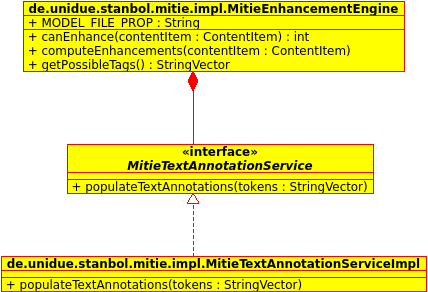
\includegraphics[width=\textwidth]{Bilder/mitie-classes.png}
\caption{''Klassendiagramm  des MITIE-Engines''}
\label{fig:mitieclasses}
\end{figure}
Die Klassen in diesem Engine spielen ähnliche Rollen, wie bei Stanford-NER mit einer gravierender Ausnahme: die Klasse \textit{NamedEntityExtractor}, die für die Extraktion von Entitäten verantwortlich ist, wird automatisch aus C++-Code erzeugt, und nicht manuell entwickelt.

\subsection{Deutcshe Korpora} \label{subsec:decor}
Nachdem die Engines, die nach Entitäten in Texten suchen sollen, entwickelt wurden, müssen die entsprechende NER-Modelle trainiert werden, wie es in der Sektion \ref{sec:trcorpora} beschrieben wurde. Und obwohl fällt dieser Schritt fürs auf Stanford-NER basierten Engine komplett aus, da dort ein vortrainiertes Modell verwendet wird, muss für weitere zwei Engines eigene Modelle trainiert werden.

Im Rahmen dieser Arbeit wurden zwei Trainingskoprora verwendet: von den Linguisten erzeugtes TIGER-Korpus und aus Basis von Wikipedia-Artikeln aufgebautes PIG-Korpus. Diese beide Korpora wurden aus folgenden Gründen ausgewählt:
\begin{itemize}
\item TIGER-Korpus wurde ausgewählt, da es das einzige deutschsprachige Korpus mit annotierten Entitäten ist, das frei verfügbar ist und das eine genügende Anzahl von Sätzen(50472 Sätzen) beinhaltet - das vom Sebastian Padó\cite{faruqui10:_training} zur Verfügung gestelltes Korpus ist zwar auch frei verfügbar, aber es beinhaltet nur 857 Sätzen, was fürs Training ungenügend ist.
\item Wikipedia wurde als Basis für automatisch aufgebautes Korpus ausgewählt, da die Dumps von Wikipedia frei verfügbar sind und eine große Anzahl von Daten (215841 Sätzen) beinhalten.
\end{itemize}

Für Training von Modellen für beide Engines (MITIE und OpenNLP) wird dasselbe Datenformat verwendet, das in der Auflistung \ref{lst:TIGEROPENBEISPIEL} beschrieben ist. Dadurch wird erreicht, dass der Code fürs Training von beiden Engines wiederverwendet werden kann.

\lstinputlisting[captionpos=b,label={lst:TIGEROPENBEISPIEL},caption={Ausschnitt aus einem Korpus im OpenNLP-Format.}]{Listings/tiger-opennlp.txt}

\subsubsection{TIGER Korpus}
\paragraph{}
TIGER-Korpus wurde von dem Institut für Maschinelle Sprachverarbeitung\cite{brants2004tiger} auf der Basis von Zeitungen aufgebaut, und beinhaltet 50474 Sätzen. Außer markierten Entitäten beinhaltet dieser Korpus auch die Informationen über POS (Part Of Speech - ob das Wort ein Verb oder ein Substantiv ist), Lemma (Infinitiv für Verben oder Nominativ Singular für Substantive) und andere Informationen über die annotierte Tokens, wie Kasus oder Genus. Der Ausschnitt des Korpuses findet man in der Auflistung \ref{lst:TIGERBEISPIEL}.

\lstinputlisting[captionpos=b,label={lst:TIGERBEISPIEL},caption={Ausschnitt aus dem TIGER-Korpus. Die Informationen, die in dieser Arbeit nicht gebraucht werden, wurden wegen Platzmangel weggelassen.}]{Listings/tiger-example.txt}
Jeder Satz ist dabei auf einer getrennter Zeile gespeichert, die Tokens werden mit Leerzeichen getrennt, und mithilfe von HTML-ähnlichen Tags werden die Entitäten markiert.

\paragraph{}
Der Korpus ist wie folgt aufgebaut:
\begin{itemize}
\item Die Sätze werden mit einer leeren Zeile getrennt.
\item Jeder Token und seine Annotationen werden in einer Zeile geschrieben. Die Spalten werden mit einem Leerzeichen getrennt.
\item Die erste Spalte beinhaltet ID des Tokens, die aus Nummer des Satzes und Nummer des Tokens innerhalb des Satzes besteht.
\item Die zweite Spalte ist der Token selbst, so wie er auch im Satz vorkommt.
\item In der dritten Spalte steht Lemma des Tokens.
\item Die vierte Spalte wird nicht verwendet.
\item Und die fünfte Spalte beinhaltet POS-Tag des Tokens. Falls dieser Tag den Typ \textit{NE} hat, ist das eine Entität.
\end{itemize}

Der Nachteil dieses Korpuses besteht darin, dass es zwischen verschiedenen Typen von Entitäten nicht unterschieden wird, und die alle den Typ \textit{NE} (NamedEntity) haben.

\paragraph{}
Die Logik, die für die Umwandlung von Tiger Korpuseinträgen in OpenNLP-Format verantwortlich ist, ist in der Auflistung \ref{lst:LOGICOFCONVERTER} zu sehen.
\lstinputlisting[captionpos=b,label={lst:LOGICOFCONVERTER},caption={Ausschnitt aus den Quelltexten des Konverters, der die Logik der Umwandlung beschreibt}]{Listings/tiger-to-onlp.java}
Es wird praktisch für jede ununterbrochene Reihenfolge von NE-Merkierungen ein OpenNLP-Tag erzeugt, und alle Wörter, die keine Entitäten sind, werden ohne Umwandlung kopiert.

\subsubsection{Wikipedia-basiertes Korpus}
\paragraph{}
Leider kann man nicht immer einen manuell aufgebauten Korpus verwenden, entweder aus Lizenz- oder Kostengründen. Viele Korpusse sind nur für Forschung frei verfügbar, was bedeutet, dass 
die auf keinen Fall in einem Geschäftsprojekt verwendet werden dürfen. Und einen eigenen Korpus aufzubauen ist auch nicht immer möglich, da dazu die Linguisten eingesetzt werden müssen, die nicht jede Firma zur Verfügung hat, und es kann Monaten dauern, bis man ein eigenes Korpus erstellt. Was könnte in diesem Fall unternommen werden?

\paragraph{}
Oliver Grisel\footnote{\url{http://www.nuxeo.com/blog/mining-wikipedia-with-hadoop-and-pig-for-natural-language-processing/}} hat einen interessanten Einsatz zur automatischer Aufbau von Korpus vorgeschlagen. Es wird vorgeschlagen, Wikipedia als Textbasis zu nehmen, und die interne Links, die auf andere Wikipediaseiten führen, sollen als  Entitäten markiert werden. Es soll anschließlich ein Korpus aufgebaut werden, auf dessen Basis ein NER-Modell trainiert werden kann. Da Wikipedia auch auf deutscher Sprache verfügbar ist, soll dieser Einsatz auch für Zwecke dieser Arbeit nützlich sein.

\paragraph{}
Um den Korpus aufzubauen, wird Apache Pig\footnote{\url{http://pig.apache.org/}} verwendet - ein Framework für Big-Data-Analyse, der eine Skript-Sprache und JavaAPI zur Verfügung stellt. Die Aufbau vom Korpus umfasst folgende Schritte:
\begin{enumerate}
\item Es wird Dump von Wikipediaartikeln heruntergeladen.
\item Es werden die Listen von Wikipedia-Links und Typen von Entitäten von DBpedia heruntergeladen. Diese Informationen braucht man später, um jeder Entität in dem erzeugten Korpus die richtige Entitätstyp zuordnen zu können.
\item Es werden Links auf interne Wikipedia-Artikeln aus Wikipedia-Dump extrahiert, mit der Positionsinformation zusammen.
\item Jeder Link wird mithilfe von DBpedia-Daten einen Entitätstyp zugeordnet.
\item Es wird ein Trainingskorpus im OpenNLP-Format erzeugt.
\end{enumerate}

\paragraph{} 
Für Korpusaufbau aus deutscher Wikipedia können im Prinzip die Scripts von Oliver Grisel genommen werden, die allerdings angepasst werden müssen:
\begin{itemize}
\item Es soll deutsche Dbpedia, und nicht englische verwendet werden.
\item Es soll deutsches Modell für Satzerkennung anstatt englisches eingesetzt werden.
\item Herunterladen von Wikipedia- und Dbpediadaten soll automatisiert werden.
\end{itemize}

Der Code, der für die Erzeugung eines Wikipedia-basierten Korpus verantwortlich ist, ist in der Auflistung \ref{app:pigcorpus} repräsentiert.

\paragraph{}
Aber welche Vor- und Nachteile hat automatische Erzeugung vom Korpus? Kann das trainierte Modell später auch tatsächlich für sinnvolle Entitätserkennung eingesetzt werden?
\begin{itemize}
\item Vorteile
\begin{itemize}
\item Die Erzeugung von Korpus braucht höchstens eine Stunde, im Vergleich zu manuell annotierten Korpora.
\item Es werden keine Fachleute gebraucht, um Korpus zu erzeugen.
\end{itemize}
\item Nachteile
\begin{itemize}
\item Nicht alle interne Links stellen eine Entität dar, und nicht alle Entitäten sind ein Link - als Folge ist die Qualität des Korpusses deutlich niedriger, als die von manuell aufgebauten.
\item Eine sehr niedrige Varianz - alle Wikipediaartikel sind mehr oder weniger in gleicher Sprache geschrieben, was bedeutet, dass wenn man dem trainierten Modell einen Text zeigt, der sich von einem durchschnittlichen Wikipedia-Artikel deutlich unterscheidet, werden da höchstwahrscheinlich keine Entitäten gefunden.
\end{itemize}
\end{itemize}

\subsection{Training von Modellen} \label{subsec:TRMODELLS}
Sowohl für OpenNLP als auch für MITIE wird Training von Modellen außerhalb von Stanbol durchgeführt. Die Ergebnisse werden dabei in den binären Dateien serialisiert, und später von entsprechenden Engines innerhalb von Stanbol geladen. Der Grund, warum es so gemacht wurde, ist die Geschwindigkeit des Trainings - wie erwähnt, erfordert Training üblich viel größere Rechnerkapazitäten als die Verwendung von Modellen selbst, bei MITIE-Engine sind das mindestens 24 GB RAM, und Training dauert aber trotzdem bis auf eine Woche. Deswegen wurde Training auf getrennten Rechnern durchgeführt.

Die Implementierung von Training an sich selbst ist relativ einfach: 
\begin{enumerate}
\item Zuerst wird die vorab erzeugte OpenNLP-Training-Datei geladen.
\item Danach wird entweder OpenNLP- oder MITIE-API aufgerufen, um ein ME- oder SVM-Modell darauf zu trainieren.
\item Am Ende wird das erzeugte Modell serialisiert und in einer Datei gespeichert.
\end{enumerate}
Das Training von einem OpenNLP-Modell ist in der Auflistung \ref{app:trainonlp} und vom MITIE-Modell in der Auflistung \ref{app:trainmitie} beschrieben.

Beim Training vom MITIE-Modell mithilfe vom Wikipedia-Korpus(PIG) musste noch folgende Anpassung gemacht werden: ursprünglich musste das ganze Korpus (215841 Sätzen) fürs Training verwendet werden, allerdings konnte das Training auf einem Rechner mit 24 GB Arbeitsspeicher nicht abgeschlossen werden, deswegen wurden für MITIE zufällige Sätze aus dem PIG-Korpus ausgewählt (71947 Sätzen), und das Modell wurde auf dieser kleineren Korpusversion traianiert.

\section{Verlinkung und Dereferinzierung von annotierten Entitäten} \label{sec:VERLINKUNGSEC}
\paragraph{}
Nachdem die Entitätserkennung durchgeführt wurde, hat man die Informationen darüber, ob es Entitäten im Text gefunden wurden, die Position der Entität innerhalb des Satzes und optional die Klasse der Entität. Die Ontologie selbst, die Endbenutzer zu sehen braucht, fehlt allerdings noch. Es müssen noch zwei Schritte durchgeführt werden, bis die Informationen komplett sind - Verlinkung von gefundenen Entitäten mit der Entitäten in einer Wissendatenbank und die Dereferinzierung von Eigenschaften der Entität.

Als Datenquelle für die Verlinkung und Dereferinzierung wird in dieser Arbeit lokaler Index von deutscher DBpedia\cite{auer2007dbpedia} verwendet. DBPedia stellt eine Kopie von Wikipedia zur Verfügung, deren Daten als RDF-Graphen gespeichert werden, und auf die mithilfe von SPARQL zugegriffen werden kann.

Während der Verlinkung von Entitäten wird für jede erkannte Entität eine Suche nach dieser Entität in einer oder mehreren Wissendatenbanken durchgeführt. Um den Vorgang höchstmöglich zu beschleunigen, soll lokaler Wissendatenbankindex (EntityHub in Terminologie von Stanbol) eingesetzt werden. Dieser Index soll vorher aufgebaut werden, und zumindest die Namen der Entitäten beinhalten. Für spätere Schritte ist aber empfehlenswert, auch diverse Eigenschaften von Entitäten zum Index hinzuzufügen, damit Dereferinzierungschritt auch so schnell wie möglich ausgeführt wird. Es muss aber beachtet werden, dass Index von realen Wissendatenbanken wie DBpedia mehr als 20 Gigabytes auf Festplattenspeicher verbrauchen kann, und die Aufbau kann mehrere Tagen in Anspruch nehmen.

Für die Verlinkung von Entitäten wird Engine ,,EntityLinkingEngine`` verwendet, dessen Aufbau auf der Abbildung \ref{fig:linking} beschrieben ist.

\begin{figure}[ht]
\centering
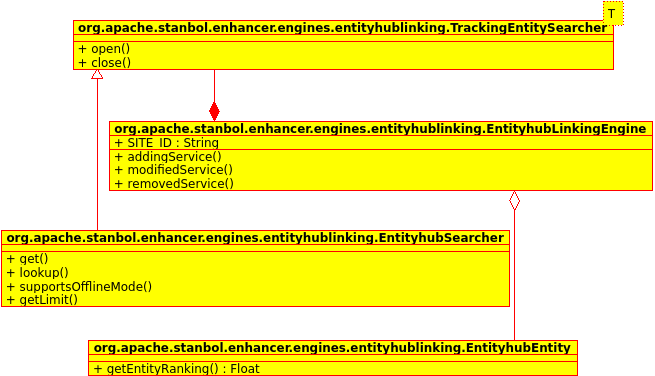
\includegraphics[width=\textwidth]{Bilder/classes-linking.png}
\caption{''UML-Klassendiagramm für EntityLinkingEngine''}
\label{fig:linking}
\end{figure}
\begin{itemize}
\item Die Klasse \textit{EntityHubSearcher}, die Interface \textit{TrackingEntitySearcher} implementiert, ist für die Suche in der Wissendatenbank zuständig.
\item Die Klasse \textit{EntityHubEntity} stellt eine Entität und ihre Eigenschaften dar. Das Parameter ,,entityRank`` zeigt, wie wichtig die Entität ist, was für die Rausfilterung von ,,unpassenden`` Entitäten helfen könnte.
\item \textit{EntityhubLinkingEngine} ist die Hauptklasse, die die Informationen über extrahierte Entitäten verlinkt.
\end{itemize}

Bei der Verlinkung von Entitäten kommt es oft vor, dass die Entitäten, die gefunden wurden, eigentlich nur Verlinkungen auf andere Entitäten, und keine selbstständige Objekten sind - z.B. die Entität ,,CDU`` ist nur ein Link auf ,,Christlich Demokratische Union Deutschlands`` ist. Solche Entitäten werden während der Verlinkung anhand der Eigenschaft ,,dbo:wikiPageWikiLink`` erkannt, und anstatt dieser Zwischenentität wird als Ergebnis der Verlinkung die referenzierende Entität verwendet.

Um die für den Benutzer relevante Informationen (Eigenschaften von Entitäten) zur Verfügung stellen zu können, müssen diese Eigenschaften aus der Datenbank geladen werden. Dazu könnte man auch direkt auf die entsprechende Schnittstelle zugreifen (http://de.dbpedia.org/resource/ für DBpedia, zum Beispiel), so ein Vorgehen würde aber zeitaufwändig und ineffektiv sein. Deswegen soll auch für die Dereferinzierung EntityHub eingesetzt werden. Für diesen Zweck wird Engine \textit{EntityhubDereferenceEngine} eingesetzt, der für jede im Verlinkungsschritt gefundene Entität alle für den Link verfügbare Eigenschaften zu dem Anreicherungsergebnis hinzufügt. Die Klassendiagramm für dieses Engine ist auf der Abbildung \ref{fig:deref} zu sehen. 

\begin{figure}[ht]
\centering
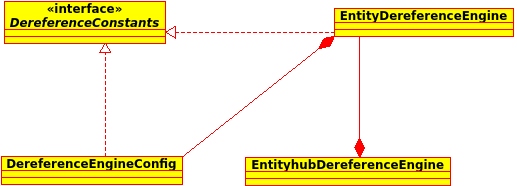
\includegraphics[width=\textwidth]{Bilder/deref-uml.png}
\caption{''UML-Klassendiagramm für EntityhubDereferenceEngine''}
\label{fig:deref}
\end{figure}
Theoretisch können hier auch SQL-Datenbanke für die Dereferenzierung verwendet werden - es muss nur eine eigene Klasse, die vor dem Interface \textit{ENtityDereferenceEngine} erbt, implementiert werden, aber wegen der möglichen Problemen, die in der Einleitung (\ref{sec:wiss}) beschrieben wurden, wäre es nicht empfohlen.

\section{Rausfilterung von für den Benutzer irrelevanten Entitäten}
Wie in der Aufgabenstellung (\ref{sec:Aufgabenstellung}) gesagt wurde, müssen nur relevante Entitäten dem Benutzer angezeigt werden, damit der Benutzer sich nicht verwirrend fühlt. Die beste Lösung dieses Problems wäre eventuell eine semantische Analyse der Benutzeranfrage, und ein Matching von Entitäten mit den Ergebnissen solcher Analyse, aber wegen Zeitmangel und einem zu großen Aufwand, der außer Rahmen dieser Masterarbeit stünde, konnte diese Lösung nicht implementiert werden. Statdessen werden folgende Gewichte verwendet, um zu entscheiden, ob eine Entität wichtig genug ist:
\begin{itemize}
\item Das Gewicht der Entität innerhalb des EntityHubs verwendet, das anhand von Anzahl der Wikipedia-Links, die auf die Entität zeigen, festgesetzt wird. Wert ,,1`` entspricht dabei dem höchstmöglichen und ,,0`` dem kleinstmöglichen Gewicht.
\item Das ,,Sicherheitswert`` (Confidence) der extrahierten Entität - wie hoch ist die Wahrscheinlichkeit $p(y|x)$ (wie in der Sektion \ref{subsec:crftheory} beschrieben), dass das Wort $x$ eine Entität der Klasse $y$ ist.
\end{itemize}

Das Engine, das diesen Filter implementiert, besteht nur aus einer Klasse, die schrittweise überprüft ob die Confidence- und Rank-Werte kleiner als in einer Konfigurationsdatei vordefinierte Schwellwerte sind. Falls ein von den beiden Werten kleiner als Schwellwert ist, wird die Entität aus der Liste von Ergebnissen gelöscht.

Die Schwellwerte für beide Filter (0.7 für Confidence und 0.2 für den Rank) wurden nach manuellem Austesten von Engines anhand persönlichen Erfahrungen des Entwicklers ausgewählt.

\section{API f{\"{u}}r Anreicherung von Suchergebnissen}
\paragraph{}
Um dem Endentwickler die Anreicherung von Suchergebnissen so einfach wie möglich zu machen, wurde eine API entwickelt, die direkt an ein beliebiges Java-Projekt als eine Bibliothek angebunden werden kann. Diese Bibliothek wird auch später in der Evaluierung verwendet. Es wurde eine Abstraktionsschicht hinzugefügt, die die Aufrufe der REST-Schnittstelle von Stanbol hinter der Klientklasse verbirgt. Der Entwickler soll nur die Liste von Suchsnippets an API übergeben, für die Verbindungaufbau zum Stanbol und Parsing der Antwort des Servers ist API verantwortlich. Die Beschreibung der API-Schnittstelle, die für den Entwickler sichtbar ist, findet man in der Auflistung \ref{lst:APISCHNITSTELLE}. 

Als Eingabedaten übergibt man die Liste von URLs gefundenen Webseiten mit dazugehörigen Texten von Snippets zusammen, und als Ausgabe bekommt man für jede URL die Liste von gefundenen Entitäten. Da in Rahmen dieser Arbeit mehr verschiedenen Engineketten implementiert wurden, muss der Name der erwünschten Kette miteingegeben werden.

Die API wurde außerdem so entworfen, dass bei Bedarf nicht nur Stanbol, sondern jedes beliebiges System als Backend verwendet werden kann - für jedes neues Backend muss nur die Klasse ,,EnhancementClient`` abgeleitet werden, und in der abgeleiteten Klasse die Schnitstelle zum neuen System implementiert werden. Gegebenfalls sollen auch neue Konverter geschrieben werden, falls Backend keine RDF-Daten liefert, und eigenes Datenformat verwendet.

Eine UML-Klassendiagramm für die Stanbol-API ist auf der Abbildung \ref{fig:apiuml} zu sehen. Es soll beachtet werden, dass die Schnitstelle zur Suchmaschine absichtlich außer Acht gelassen wurde - um die API so generisch wie möglich zu gestalten, wird die Anbindung an Suchmaschine dem Entwickler, der die API verwendet, überlassen. 

\begin{figure}[ht]
\centering
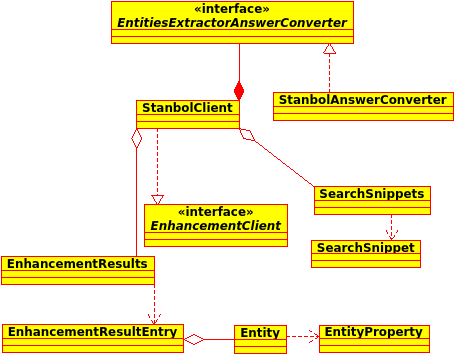
\includegraphics[width=\textwidth]{Bilder/apiuml.png}
\caption{''Struktur der Stanbol-API''}
\label{fig:apiuml}
\end{figure}
\begin{itemize}
\item Die Klasse \textit{StanbolClient} implementiert das Interface \textit{EnhancementClient}, und spielt die Rolle der Hauptklasse für die Konversation mit Stanbol.
\item \textit{StanbolAnswerConverter} umwandelt die Antwort des Stanbol-Servers (RDF) in das interne API-Format:
\begin{itemize}
\item Die Klasse \textit{EnhancementResults}, die als ein Container für gefundene Entitäten dient.
\item Die Klasse \textit{EnhancementResultEntry}, die die  Ergebnisse der Extraktion für eine bestimmte Webseite zusammenfasst.
\item \textit{Entity}, die eine Entität mit den Parametern zusammen (als eine Liste von \textit{EntityProperty}) darstellt.
\end{itemize}
\item Die Klassen \textit{SearchSnippets} und \textit{SearchSnippet} werden für die Zwischenspeicherung von den Snippets und URLs, die eine Suchmaschine geliefert hat, verwendet. Die Schnittstelle zu der Suchmaschine wird von dem Entwickler implementiert.
\end{itemize}
\chapter{Evaluierung}

\section{Benutzerevaluierung}
\paragraph{}
Damit es festgestellt werden könnte, ob die Anreicherung von Suchergebnissen mit aus den Snippets extrahierten Entitäten für den Benutzer auch tatsächlich hilfreich sein könnte, wurde eine Benutzerevaluierung durchgeführt. Die Evaluierung soll bei der Überprüfung von folgenden Hypothesen helfen:

\begin{itemize}
\item Die in den kurzen Suchsnippets vorhandene Informationen könnten für die Extraktion von Entitäten nicht ausreichend sein, und es müsste eventuell auf den kompletten Text der referenzierten Webseite zugegriffen werden.
\item Die Präzision und Sensitivität des Engines könnten einen großen Einfluss darauf haben, wie gut sich das Engine für die Benutzerunterstützung eignet.
\item Die in den verlinkten Entitäten vorhandene Informationen, die aus der DBpedia extrahiert wurden, könnten einen größeren Einfluss auf die Zufriedenheit des Benutzers haben als die Präzision des Engines.
\item Die Geschwindigkeit der Suche könnte durch den zusätzlichen Schritt der Extraktion von Entitäten stark beeinträchtigt werden, was den Benutzer bei der Suche stören würde.
\end{itemize}

Um diese Hypothesen bestätigen oder widerlegen zu können, wurde eine Webseite aufgebaut, die dem Benutzer die Möglichkeit gibt, alle im Rahmen dieser Arbeit entwickelte Engines und alle Modellen, die im Rahmen dieser Arbeit verwendet wurden, zu bewerten. 

Für jedes Engine sollen insgesamt drei Charakteristiken bewertet werden:
\begin{enumerate}
\item Qualität von extrahierten Entitäten - der Benutzer soll bewerten, wie gut seiner Meinung nach die extrahierte Entitäten zu den gefundenen Textsnippets passen, ob diese ,,korrekt`` von dem Gesichtspunkt des Probanden waren, ob es für die gefundene Entitäten die Eigenschaften vorhanden sind, die der Benutzer auch wirklich braucht, und ob die extrahierte Entitäten die Informationen beinhalten, die bei der Suche nicht weiter helfen können.
\item Geschwindigkeit der Anreicherung - der Proband soll angeben, ob die Extraktion von Entitäten mit der Suche zusammen schnell genug waren, besonders im Vergleich zu den Suchmaschinen wie Google oder Bing.
\item ,,Hilfreichsgrad`` von dem Ansatz - damit soll der Benutzer mitteilen, ob solch eine Anreicherung von herkömmlichen Suchergebnissen mit den Entitäten und dazugehörigen Informationen wie Geburtstag/Geburtsort/usw. für die Präzision der Suchanfrage hilfreich wäre, und ob der Proband den Einsatz dieser Suchmethode sinnvoll fände. 
\end{enumerate}
Jede Charakteristik soll mit einem Wert von ,,1`` (ungeeignet) bis ,,5`` (ausgezeichnet) bewertet werden. Dabei sollen die o.g. Charakteristiken bei der Überprüfung der am Anfang des Kapitels gestellten Hypothesen wie folgt helfen:
\begin{enumerate}
\item Die Bewertung der Geschwindigkeit des Engines hilft zu überprüfen, ob die Geschwindigkeit der Suche mit der Erkennung von Entitäten tatsächlich viel kleiner als die der herkömmlichen Suche ist.
\item Zwei weitere bewertete Charakteristiken mit den Ergebnissen der systemorientierten Evaluierung (Siehe die Sektion \ref{sec:sysevalsec}) zusammen helfen bei der Überprüfung der Aussagen über die Korrelationen zwischen Sensitivität, Präzision und der Nutzbarkeit des Engines für die Benutzerunterstützung.
\end{enumerate}

Während der Evaluierung muss der Benutzer alle vorhandene Kombinationen von Algorithmen und verwendeten Modellen nacheinander bewerten, in sieben Schritten. Die Bewertung gilt nur dann als gültig, wenn der Benutzer \textbf{alle vorhandene} Kombinationen bewertet hat, ansonsten gilt die Bewertung als ,,ungültig``, und wird daher nicht berücksichtigt.

Diese Einschränkung wurde eingeführt, da einige Benutzer (7 Sessionen insgesamt) die Evaluierung nach dem zweiten oder dritten Schritt abgebrochen haben. Hätte man diese Bewertungen miteinkalkuliert, hätten einige Kombinationen von Engines und Modellen mehr Bewertungen erhalten als die andere, und für genauere Ergebnisse sollen die Bewertungen \textbf{gleichmäßig} zwischen allen Engines verteilt werden.

Die Aufbau der Evaluierungsseite lässt sich in vier Bereiche teilen:

Im ersten Bereich (siehe die Abbildung \ref{fig:eval-select-question}) soll die Anfrage, die Benutzer stellen möchte, ausgewählt werden. Dabei kann der Benutzer in diesem Schritt keine beliebige Frage stellen. Stattdessen muss eine der vorgegebenen Fragen ausgewählt werden. Dadurch wird erreicht, dass jeder Benutzer die gleichen Fragen zum Auswahl hat, was bedeutet, dass auch die Antworten, die der Server dem Benutzer anzeigt, für jeden Benutzer gleich sein werden. Damit wird sichergestellt, dass jeder Benutzer die gleichen Ausgangsdaten bewertet, ansonsten hat man die Situation, wenn die Benutzer anfangen, die Fragen und nicht das Engine zu bewerten. Außerdem soll die Anzahl von den für den Benutzer verfügbaren Freiheitsgraden so klein wie möglich sein, damit die Wahrscheinlichkeit, dass der Benutzer einen Fehler macht, gering gehalten werden könnte.

\begin{figure}
\centering
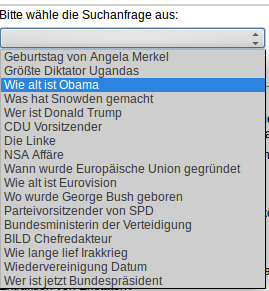
\includegraphics[width=.6\textwidth]{Bilder/select-question.png}
\caption{''Auswahl einer Frage''}
\label{fig:eval-select-question}
\end{figure}

Dabei wurden die Fragen in zwei Gruppen geteilt, um mögliche Abhängigkeit der Ergebnisse von dem Domain erkennen zu können - da verschiedene Engines und Modelle auf verschiedenen Korpora trainiert wurden, kann es sein, dass z. B. die Modelle, die auf Zeitungen trainiert wurden (TIGER Korpus), auch bei den Zeitung-ähnlichen Texten besser abschneiden werden. Es wurden folgende Gruppen von Fragen verwendet:
\begin{enumerate}
\item Die Fragen, die zum Domain ,,Zeitungen`` passen, was bedeutet, dass die Suchmaschinen bei der Beantwortung dieser Fragen höchstwahrscheinlich die Links auf Online-Zeitungen zurückgeben werden.
\item Die Fragen, die zum Domain ,,Web/Wikipedia`` passen, was bedeutet, dass die Suchmaschinen bei der Beantwortung dieser Fragen die Links auf Wikipedia zurückgeben sollen.
\end{enumerate} 
Um gleiche Bedeckung von allen möglichen Kombinationen von Domains und Fragegruppen zu gewährleisten, wird es bei jedem Engine zwischen verfügbaren Fragegruppen zyklisch gewechselt - für den ersten Benutzer wird die Reihenfolge 'Domain1/Engine1 $\longrightarrow$ Domain2/Engine2 $\longrightarrow$ Domain1/Engine3 ...' verwendet, für den zweiten 'Domain2/Engine1 $\longrightarrow$ Domain1/Engine2 $\longrightarrow$ Domain2/Engine3 ...' usw.

Nachdem der Benutzer die gewünschte Frage ausgewählt und gestellt hat, wird ihm im zweiten Bereich, dessen Screenshot auf der Abbildung \ref{fig:eval-entitylist} zu sehen ist, eine Liste von gefundenen Snippets mit den verlinkten Entitäten zusammen angezeigt.

\begin{figure}
\centering
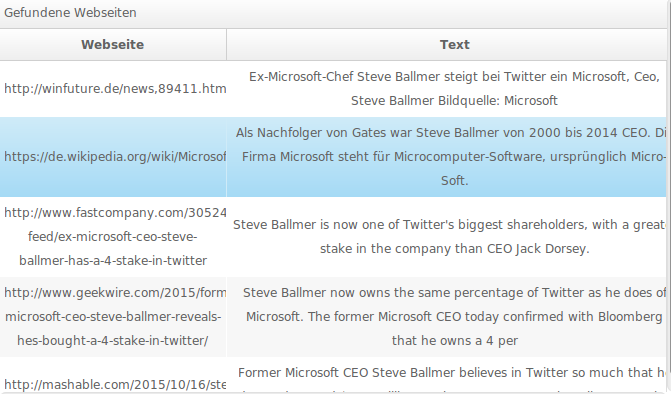
\includegraphics[width=1\textwidth]{Bilder/evalstep02-step1.png}
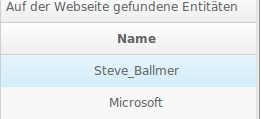
\includegraphics[width=0.5\textwidth]{Bilder/evalstep02-step1-2.png}
\caption{''Liste von Snippets und gefundenen Entitäten''}
\label{fig:eval-entitylist}
\end{figure}

Die Links und dazugehörige Snippets kommen dabei direkt vom Bing, und werden damit von der Implementierung eines Engines nicht beeinflusst. Die Liste von den extrahierten Entitäten wird dagegen von dem Stanbol erstellt. Die Snippets, wo keine Entitäten gefunden werden konnten, werden in der Liste nicht angezeigt.

Im dritten Bereich (siehe die Abbildung \ref{fig:eval-props}) werden die Eigenschaften der ausgewählten Entität angezeigt. In der linken Spalte wird der Name der Eigenschaft abgebildet und rechts das Wert. Es gibt dabei zwei verschiedene Typen von Werten:
\begin{itemize}
\item ,,Rohe`` Eigenschaften, wie Geburts- oder Todesdatum oder Kurzbeschreibung. Diese sind im Prinzip Zeichenketten und können dem Benutzer ohne weiteres angezeigt werden.
\item ,,Links`` - das sind die Eigenschaften, die eigentlich nur Links auf andere Entitäten sind, die ihre eigene Eigenschaften besitzen. Zum Beispiel ist Geburtsort einer Person ein Link auf entsprechendes DBpedia-Eintrag, dasselbe gilt auch für Sprache oder sogar Zeitzonen.
\end{itemize}

Im letzten Bereich soll das getestete Engine bewertet werden, wie es auf der Abbildung \ref{fig:bewertung} angezeigt wird.

Nachdem alle Kombinationen getestet wurden, wird dem Benutzer die Möglichkeit gegeben, eine beliebige Frage an ein Engine zu stellen und einen persönlichen Feedback abzugeben. Die Aufbau dieser letzten Seite ähnelt sich der von der Seite, wo ein Engine bewertet wird, mit dem Unterschied, dass anstatt der Form für die Bewertung wird im letzten Bereich die Form für den Feedback und das Eingabefeld für die beliebige Frage angezeigt. Diese Änderung ist auf dem Screenshot \ref{fig:finish-eval} zu sehen. Diese Form wurde eingeführt, um die Anregungen für mögliche Verbesserungen vom Backend und für Nachfolgerarbeit sammeln zu können.

Während der Studie wurden insgesamt 44 Bewertungen gesammelt, deren Ergebnisse in der Tabelle \ref{app:RESULTS} zu sehen sind. Es wurden außerdem einige Feedbacks gesammelt, die für die Analyse der Arbeit und als Quelle für Verbesserungsvorschläge verwendet werden können. Die Liste von Feedbacks findet man in der Auflistung \ref{app:feedbacks}.

\begin{table}
\begin{tabular}{|c|c|c|c|c|}
\hline 
• & helpQuality & quality\_newspapers & quality\_misc & speed \\ 
\hline 
mitie-nerchain-pig & 3.23 & 1.98 & 1.45 & 4.09 \\ 
\hline 
mitie-nerchain-tiger & 3.15 & 1.25 & 2.09 & 3.8 \\ 
\hline 
pig-nerchain & 3.05 & 1.31 & 2 & 3.87 \\ 
\hline 
stanford-nerchain-both & 3.07 & 1.23 & 1.95 & 4.05 \\ 
\hline 
stanford-nerchain-dewac & 3.25 & 2.11 & 1.41 & 4.16 \\ 
\hline 
stanford-nerchain-hgc & 3.11 & 1.34 & 1.86 & 4.16 \\ 
\hline 
tiger-nerchain & 3.34 & 1.93 & 1.39 & 3.98 \\ 
\hline 
\end{tabular} 
\caption{Ergebnisse der Benutzerevaluierung}
\label{app:RESULTS}
\end{table}

Die Erklärung und Auswertung von den gesammelten Ergebnissen wird später in der Sektion ,,Diskussion`` (\ref{sec:diskussion}) vorgeführt. 

\section{Technische Implementierung der Benutzerevaluierung}
\paragraph{}
Die Komponentenstruktur der Evaluierungsseite ist auf der Abbildung \ref{fig:evalcomponents} dargestellt. Das System besteht insgesamt aus folgenden Komponenten:
\begin{enumerate}
\item Die Evaluierungswebseite selbst ist als eine Java-Webapplikation implementiert, und ist für die graphische Oberfläche verantwortlich.
\item Die Bing-API, die im Rahmen der Masterarbeit von Karatassis\cite{Karatassis:15} entwickelt wurde, stellt eine Schnittstelle zur Suche im Bing zur Verfügung.
\item MongoDB - eine dokumentenbasierte NoSQL-Datenbank - dient als Quelle für verfügbare Fragen und speichert außerdem die Bewertungen und Feedbacks von Benutzern.
\item Mit Hilfe der API für Extraktion von Entitäten greift die Webseite auf Stanbol, der auf einem anderen Rechner läuft, über eine REST-API zu. 
\end{enumerate}

\begin{figure}
\centering
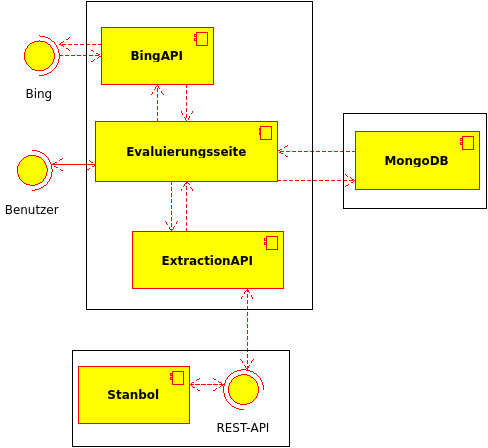
\includegraphics[width=1\textwidth]{Bilder/evaluation_components.png}
\caption{''Komponentendiagramm der Evaluierungsseite''}
\label{fig:evalcomponents}
\end{figure}
Der Vorteil dieser Architektur ist, dass die sich auf mehrere Rechnern verteilen lässt, womit die Verfügbarkeit und Belastbarkeit des System erhöht werden könnte.

Technische Details der Ablauf der Evaluierung werden auf der Diagramm \ref{fig:eval-ablauf} abgebildet. Der Vorgang der Evaluierung lässt sich in folgende Schritte aufteilen:
\begin{enumerate}
\item Zuerst wird die Anfrage des Benutzers an Web-Frontend gesendet.
\item Danach wird diese Anfrage an Bing weitergeleitet. Der BingAPI wird dabei mitgeteilt, dass bei Möglichkeit nur nach deutschsprachigen Webseiten gesucht werden muss.
\item Die Liste von Links auf gefundene Webseiten mit den Texten von Snippets zusammen, die vom Bing erhalten wurden, wird über ExtraktionAPI an Stanbol weitergeleitet.
\item Die von dem Stanbol erhaltene Antwort wird mithilfe von der ExtraktionAPI aus RDF in Java-Objekte transformiert.
\item Die Evaluierungsseite serialisiert extrahierte Entitäten, fügt die der vom Bing erhaltener Liste von Snippets zu und sendet die Ergebnisse an den Benutzer.
\item Der Benutzer benutzt Webseite-UI um das Engine zu bewerten.
\item Die Bewertung wird in der Datenbank gespeichert, und Benutzer kann mit dem nächsten Engine fortfahren.
\end{enumerate}

\begin{figure}
\centering
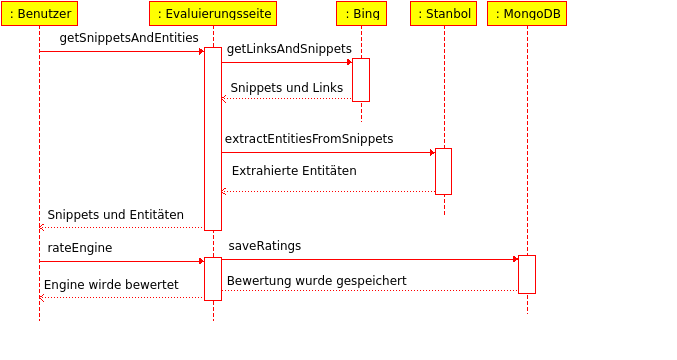
\includegraphics[width=1\textwidth]{Bilder/eval_sequence.png}
\caption{''Ablauf der Evaluierung''}
\label{fig:eval-ablauf}
\end{figure}

Die auf der Abbildung \ref{fig:evalcomponents} dargestellte Komponenten werden durch folgende Klassen implementiert:
\begin{itemize}
\item Das Interface \textit{EvaluationSessionService} und implementierende Klasse \textit{EvaluationSessionServiceImpl} sind für die Steuerung des Evaluierungsvorgangs zuständig:
\begin{itemize}
\item Die starten und beendet die Evaluierung für einen bestimmten Benutzer.
\item Die wechseln zum nächsten Engine, wenn der Benutzer die Bewertung abgeschickt hat.
\item Die leiten die Benutzerbewertungen und Anfragen zu anderen Komponenten weiter.
\end{itemize}
\item \textit{EingineRatingService} ist für die Speicherung von Benutzerbewertungen zuständig. Dabei definiert das Interface nicht, wie genau die Daten gespeichert werden - es muss also nicht unbedingt eine NoSQL datenbank sein - es wird nur eine generische Schnittstelle für Abgabe von Bewertungen zur Verfügung gestellt.
\item Die Klasse \textit{EingineRatingServiceMongoImpl} ist die Implementierung der \textit{EingineRatingService}-Schnittstelle für MongoDB.
\item \textit{MongoDbClient} stellt eine Abstraktion über die Mongo Java API zur Verfügung, damit es weniger Code für andere Klassen geschrieben werden müsste.
\item Die Klassen \textit{MongoFeedbackService} und \textit{AvailableQueriesFromDatabaseServiceMongoImpl} sind entsprechend für die Speicherung von Benutzerfeedbacks und möglichen Evaluierungsanfragen zuständig. 
\item \textit{EntityExtractionService} ruft zuerst Bing API (implementiert durch die Klasse \textit{BingSearchService}) auf, um die Liste von gefundenen Snippets für die angegebene Suchanfrage liefern zu lassen. Danach wird die Extraktion-API aufgerufen, um die gefundene Snippets mit Entitäten anzureichern. Die Ergebnisse werden zurück an \textit{EvaluationSessionService} geschickt.
\item Die Schnittstelle \textit{QueryLogService} und ihre Implementierung \textit{QueryLogServiceMongoImpl} sichern die Anfragen, die Benutzer im letzten Schritt der Evaluierung gesendet haben.
\end{itemize}

%\begin{figure}
%\centering
%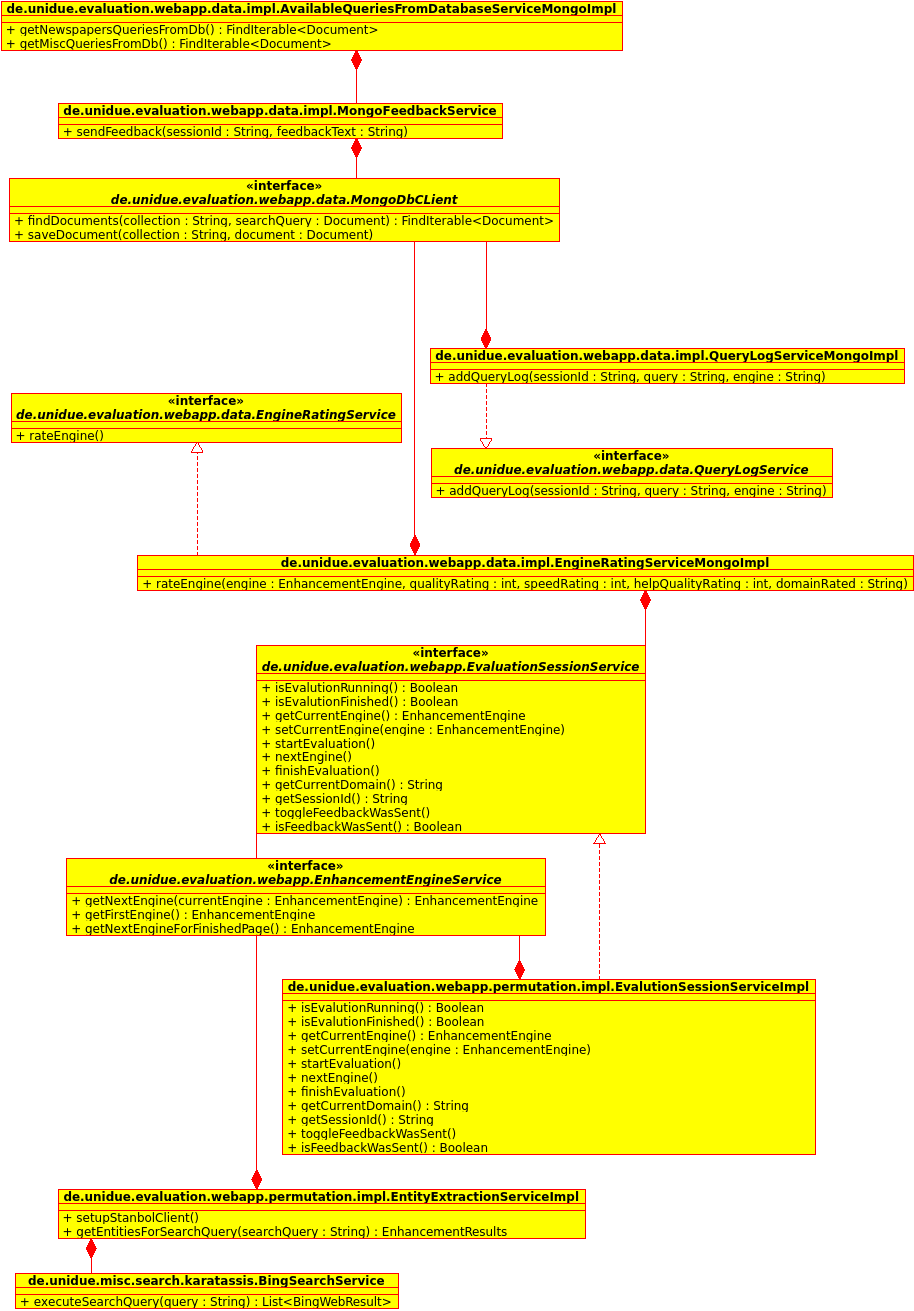
\includegraphics[width=1\textwidth]{Bilder/eval_classes.png}
%\caption{''Klassendiagramm der Evaluierungsseite''}
%\label{fig:evalclasses}
%\end{figure}

Genau wie Stanbol kann die Evaluierungsseite auf jedem Java Applikationsserver gestartet werden. Es ist möglich, dass die Seite eine Java VM mit Stanbol teilt, was allerdings aus Geschwindigkeitsgründen nicht empfohlen wird.

\section{Systemorientierte Evaluierung von Qualität der Extraktion} \label{sec:sysevalsec}
\paragraph{}
Bevor die Ergebnisse der Benutzervaluierung bewertet werden können, muss geprüft werden, wie präzis die Engines Entitäten erkennen können. Da ein Engine in seiner Funktionsweise ein Klassifikator ist (siehe Kapitel ,,Grundlagen``, Sektion \ref{sec:Grundlagen}), kann die Präzision eines Engines anhand von folgenden Metriken bestimmt werden\footnote{\url{https://de.wikipedia.org/wiki/Beurteilung_eines_Klassifikators\#Wahrheitsmatrix:_Richtige_und_falsche_Klassifikationen} (Zuletzt abgerufen am 05. November)}
\begin{enumerate}
% dund  (die Wörter, die keine Entitäten sind, und die nicht als Entitäten annotiert wurde) definiert werden.
\item Anzahl von False-Positive-Treffer - die von dem Engine als Entitäten erkannte Wörter, die keine Entitäten sind.
\item Anzahl von True-Positive-Treffer - die Entitäten, die von dem Engine als solche erkannt wurden.
\item Anzahl von True-Negative-Treffer - die Wörter, die keine Entitäten sind, und die als solche nicht annotiert wurden.
\item Anzahl von False-Negative-Treffer - die von dem Engine nicht erkannte Entitäten.
\end{enumerate}

Die oben genannte Zahlen können mithilfe von folgenden Metriken zusammengefasst werden\cite{och2003systematic}:
\begin{itemize}
\item Präzision beschreibt den Anteil von True-Positive-Treffer an allen als Entitäte markierten Wörtern (die Summe von True-Positive- und False-Positve-Treffer).
\item Sensitivität (Recall) beschreibt den Anteil von korrekt als Entitäte erkannten Wörtern (True-Positive-Treffer) an den Anzahl von allen im Text vorhandenen Entitäten (Die Summe von True-Positive-Treffer und False-Negative-Treffer).
\item F-Measure fasst Präzision und Sensitivität mithilfe des gewichtetes harmonisches Mittels zusammen. Die Formel für die Kalkulation von F-Maß für Präzision $P$ und Sensitivität $S$ sieht wie folgt aus\cite{hripcsak2005agreement}:
$$
F=\frac{(1+\beta^2)*S*P}{(\beta^2*P)+S}
$$ 
Die Variable $\beta$ bestimmt dabei, was ein höheres Gewicht für die Kalkulation des F-Wertes hat: Präzision oder Sensitivität. Allerdings sollen diese beide Maßen in meisten Fällen laut Hripcsak\cite{hripcsak2005agreement} gleiches Gewicht besitzen, und so kann das Gewicht $\beta$ auf $1$ gesetzt werden.
\end{itemize}

Nachdem die Maßen, die für jedes Engine berechnet werden sollen, definiert wurden, muss ein Verfahren zur Beurteilung von Engines bestimmt werden (das bedeutet, dass es eine Methodik ausgewählt werden soll, die bestimmt, wie die Evaluierung durchgeführt werden soll). In der Arbeit von Kovahi et al.\cite{kohavi1995study} wurde erwähnt, dass zur Bewertung von Klassifikatoren Kreuzvalidierung verwendet werden soll. Allerdings kann die Kreuzvalidierung nicht auf alle Engines angewendet werden, da es für einige Engines keine Trainingskorpora zur Verfügung stehen, wie es im Kapitel ,,Implementierung`` (Sektion \ref{subsec:stanfordner}) erwähnt wurde. Aus diesem Grund wird in dieser Masterarbeit folgende Evaluierungsmethodik verwendet:
\begin{itemize}
\item Als Musterdaten für die Evaluierung wurden TIGER- und PIG-Korpora verwendet:
\begin{itemize}
\item Die Engines, die mithilfe von PIG trainiert wurden, werden mit dem TIGER-Korpus ausgetestet.
\item Die Engines, die mithilfe von TIGER trainiert wurden, werden mit dem PIG-Korpus ausgetestet.
\item Auf Stanford-NER aufgebaute Engines wurden mithilfe von PIG-Korpus getestet, da er größer ist, und da die Varianz von Daten dort größer sein soll, und so theoretisch genauere Ergebnisse liefern könnte.
\end{itemize}
\item Die Anfragen werden direkt an eine Stanbol-Instanz mithilfe der REST-API gesendet.
\end{itemize}
Auf diese Art und Weise wird nicht nur die Qualität von den verwendeten Modellen bewertet, sondern auch andere Bestandteile von Engines, wie Filter von Entitäten und Verlinkung- und Dereferenzierungsengines.

Die Ergebnisse dieser systemorientierter Evaluierung sind in der Tabelle \ref{tab:AUTOEVAL} aufgelistet. Es lässt sich gut erkennen, dass die Ergebnisse sich mit den im Kapitel ,,Grundlagen`` (Sektion \ref{sec:Grundlagen}) gemachten Annahmen gut vereinbaren lassen - das Engine, das SVM als Basisalgorithmus verwendet (MITIE), zeigt auch die beste Ergebnisse. Aber wie gut spiegeln diese Daten die ,,Zufriedenheit`` der Benutzer mit dem Engine? Auf diese Frage wird während der Diskussion von Ergebnissen (\ref{sec:diskussion}) angegangen.

\begin{table}
\begin{tabular}{|c|c|c|c|}
\hline 
• & F-Measure & Recall & Präzision \\ 
\hline 
MITIE (PIG) & 0.585 & 0.506 & 0.693 \\
\hline
OpenNLP (PIG) & 0.404 & 0.299 & 0.621 \\
\hline
STANFORD (deWac+hgc) & 0.246 & 0.187 & 0.359 \\
\hline
STANFORD (deWac) & 0.280 & 0.219 & 0.390 \\
\hline
STANFORD (hgc) & 0.271 & 0.209 & 0.388 \\
\hline 
MITIE (TIGER) & 0.557 & 0.624 & 0.503 \\
\hline
OpenNLP (TIGER) & 0.409 & 0.357 & 0.479 \\
\hline
\end{tabular} 
\caption{Ergebnisse der systemorientierten Evaluierung}
\label{tab:AUTOEVAL}
\end{table}

\section{Diskussion} \label{sec:diskussion}
\paragraph{}
Nachdem sowohl system- als auch benutzerorientierte Evaluierungen durchgeführt wurden, können die Ergebnisse zusammengefasst und erklärt werden. Auf den ersten Blick lassen sich aus den vorgestellten Ergebnissen folgende Schlussfolgerungen ziehen:
\begin{itemize}
\item Die Benutzer fanden den Einsatz hilfreich, wünschen sich aber die Verbesserung von dem Benutzerinterface des Systems.
\item Es werden eventuell zu viel Informationen angezeigt, so dass der Benutzer sich verwirrt fühlen könnte.
\item Die Probanden fanden die Geschwindigkeit der Suche gut, auch wenn es definitiv länger als eine Suche mit herkömmlichen Suchmaschinen dauert. 
\item Die Benutzer bewerteten die Qualität von extrahierten Entitäten meistens als ,,nicht ausreichend``.
\item Obwohl die automatisierte Evaluierung von Engines klare Ergebnisse geliefert hat, und zwar, dass ein Engine viel bessere Ergebnisse gezeigt hat, als die andere, wird das in der Benutzerevaluierung nicht widergespiegelt.
\end{itemize}

Es stellt sich die Frage, was bedeuten diese Ergebnisse, und was man daraus lernen kann, und welche Aspekte des entwickelten Systems sich verbessern lassen.

Die interessanteste Frage wäre, warum die Benutzer einerseits die Qualität von den extrahierten Entitäten als ,,schlecht`` bewertet haben, aber anderseits den Einsatz von Entitäten als ,,hilfreich`` bezeichneten, und welchen Zusammenhang zwischen diesen beiden Kriterien besteht? 

Um diese Frage beantworten zu können muss es zuerst über die Definition von ,,Qualität`` von Entitäten im Rahmen der Evaluierung nachgedacht werden. In der Einleitung zur Evaluierung wurde Qualität als ,,wie gut \textbf{aus Sicht des Probanden} die Entität zu den gefundenen Snippets passt`` definiert. Das Problem hier ist, dass verschiedene Benutzer verschiedene persönliche Definitionen von den Begriffen ,,passend`` und ,,unpassend`` haben - z.B. wird aus einem Snippet zur Anfrage ,,Geburtstag von Angela Merkel`` auch die Entitäten ,,Deutschland`` und ,,CDU`` extrahiert, neben der Entität ,,Angela Merkel``, die für die Beantwortung der Anfrage eigentlich ausreichend wäre. Einige Probanden können die zwei zusätzliche Entitäten als ,,passend`` einstufen, da die zum Themengebiet des Snippet-Textes passen, aber andere Benutzer würden dieselbe Daten als ,,unpassend`` bezeichnen, da die keine Antwort auf die gestellte Frage geben. Außerdem sind die Methoden zur Extraktion von Entitäten nicht perfekt, und können im Text vorhandene Entitäten nicht immer richtig erkennen. Die Rolle vom Trainingskorpus soll auch im Kauf genommen werden - automatisch generierte Korpora sollen generell nur dann verwendet werden, wenn keine weitere Korpora verfügbar sind (aus finanziellen Gründen z.B.).

Ein weiteres Problem kann auf die Suchmaschine zurückgeführt werden, die als Quelle für Snippets verwendet wird - auch wenn in den Suchparametern der Suchmaschine explizit mitgeteilt wird, dass es nach deutschsprachigen Seiten gesucht werden muss, werden oft auch englischsprachige Webseiten gefunden, und da das im Rahmen dieser Arbeit entwickeltes System nur für deutsche Sprache funktionieren soll, werden nicht alle von der Suchmaschine erhaltene Ergebnisse mit den Entitäten angereichert.

Die Andere Quelle für die Bewertung von extrahierten Entitäten als ,,unpassend`` können die in den dem Benutzer gezeigten Ontologien vorhandene Informationen sein. Als Erstes haben einige Benutzer bemerkt, dass es auch die Eigenschaften angezeigt werden, die mit der eigentlichen Suchanfrage nichts gemeinsames haben - z.B. auch wenn man die Informationen übers Geburtsort einer Person sucht, werden für die extrahierte Entität alle in der Wissendatenbank vorhandene Informationen angezeigt - Geburtstag, Name, Beschreibung u.s.w. Das kann zur Verwirrung führen, und somit wird die Entität als ,,schlecht`` eingestuft. Zweitens, sind die in DBpedia vorhandene Daten nicht immer vollständig - bei den Daten fürs indische Ozean fehlen z.B. die Angaben zur Fläche, da die direkt in der Kurzbeschreibung der Entität zu finden sind. Das kann eventuell dazu führen, dass der Benutzer sich in die Beschreibung der extrahierten Entität einlesen muss, und somit mehr Aufwand für die Suche anzuwenden braucht als es vorgesehen wurde. 

Ein weiterer Grund, warum die Entitäten als ,,nicht ausreichend gut`` bewertet wurden, könnte das User-Interface des Bewertungssystems sein - da das Ziel dieser Arbeit die Entwicklung des Backeds und der API für die Extraktion von Entitäten aus Suchergebnisseiten war, und die UI nur für die Durchführung der Evaluierung entwickelt wurde, wurde eine grundlegende Untersuchung, wie die Daten dem Benutzer am Besten angezeigt und dargestellt werden könnten, absichtlich nicht durchgeführt, damit der Zeitplan eingehalten werden könnte. Und obwohl es gebeten wurde, nicht die UI, sondern nur die Extraktion von Entitäten an sich selbst zu bewerten, beeinflusst die UI die Entscheidung des Benutzers trotzdem. 

Die mögliche Schreibfehler sowohl in den Anfragen von Benutzern als auch in den Texten von gefundenen Snippets müssen auch im Kauf genommen werden - das System hat zur Zeit keine Möglichkeit, Schreibfehler zu korrigieren, was dazu führen kann, dass einige vorhandene Entitäten nicht gefunden werden.

Anschließend könnte auch die Komplexität der Evaluierungsseite an sich selbst auf den Benutzer verwirrend wirken, und so für schlechtere Wahrnehmung der Ergebnissen sorgen.

Der Grund für die Unstimmigkeiten zwischen der Benutzer- und automatisierten Evaluierung könnte die Tatsache sein, dass für den Benutzer \textbf{die in den Entitäten vorhandene Daten}, wie Geburtsort, viel wichtiger, als die Entitäten selbst sind - auch wenn eine Entität aus dem Text extrahiert wurde, kann die für den Benutzer ohne verlinkte Eigenschaften nicht nützlich sein.

\chapter{Fazit}

\section{Zusammenfassung}
Im Rahmen dieser Arbeit wurden verschiedene Methoden zur Extraktion von Entitäten aus natürlichsprachlichen Texten untersucht und miteinander verglichen. Es wurden außerdem verschiedene Datenquellen für Trainingskorpora verglichen, sowohl mithilfe von den Linguisten als auch automatisch erzeugte. Es wurde anschließend eine Erweiterung für das Stanbol-Framework entwickelt, die die Extraktion von Entitäten aus deutschsprachigen Suchergebnisseiten ermöglicht und es wurde eine Benutzerevaluierung durchgeführt, die zeigen sollte, ob die Extraktion von Entitäten den Benutzer bei der Suche tatsächlich unterstützen könnte. 

Die Untersuchung von möglichen Algorithmen der Extraktion von Entitäten hat gezeigt, dass die Algorithmen, die sonst für Klassifizierung verwendet werden, auch für die NER-Aufgabe eingesetzt werden können - es müssen lediglich korrekte ,,Eigenschaften`` von Wörtern (Features) ausgewählt werden, mit deren Hilfe dem Wort eine Klasse zugeordnet werden könnte. Dabei müssen die Eigenschaften nicht unbedingt von Menschen definiert werden (supervised Features), sondern können auch automatisch berechnet werden (unsupervised Features).

Die Wichtigkeit von einem richtigen Training-Korpus für eine erfolgreiche Erkennung von den Entitäten lässt sich nicht von der Hand zu weisen - es ist sehr wichtig, dass das verwendete Korpus folgende Eigenschaften besitzt:
\begin{enumerate}
\item Groß genug ist, damit das Modell genug Daten fürs Training hat.
\item Gute Qualität hat - das bedeutet, dass alle Entitäten, die im Korpus vorkommen, auch wirklich markiert sind, und zwar richtig (eine Person soll als eine Person, und nicht als eine Firma annotiert werden), dass die Sätze korrekt getrennt sind, dass es keine nicht-Entitäten markiert werden.
\item Aus dem zweiten Punkt folgt, dass das Korpus im besten Fall von Linguisten erstellt sein soll.
\end{enumerate}

Leider erfüllen die frei verfügbare Korpora fast immer nur das erste Kriterium - einige von denen sind automatisch generiert, bei anderen fällt die Unterscheidung zwischen verschiedenen Typen von Entitäten komplett aus und es nur bekannt ist, ob ein bestimmtes Token eine Entität ist, die Klasse bleibt aber unbekannt. Diese Einschränkung hat selbstverständlich auch diese Arbeit beeinflusst, und die Qualität von dem Framework war eigentlich schlechter als die sein könnte. Deswegen soll bei akademischen Werken auch ökonomische Faktoren berücksichtigt werden - da frei verfügbare Korpora nicht unbedingt eine gute Qualität aufzeigen können, sollte gelegentlich eine Option der Finanzierung eines passenden Korpus im Kauf genommen werden. 

Die Benutzerstudie hat gezeigt, dass der Einsatz von Entitäten bei der Websuche für den Benutzer theoretisch hilfreich sein könnte, allerdings muss sowohl Framework (Backend) als auch User-Interface (Frontend) weiter entwickelt und verbessert werden, um eine genügende Unterstützung bei der Suche gewährleisten zu können. Es wurde festgestellt, dass die in den Entitäten vorhandene Informationen für den Benutzer nicht nur hilfreich, sondern auch störend sein können, falls es zu viele davon gibt.

Das Training eines Modell für Erkennung von Entitäten stellt eine getrennte Aufgabe dar, die bei einigen Algorithmen (SVM) einen großen Rechenaufwand benötigt und bis auf mehrere Tagen in Anspruch nehmen kann. Und generell ist das Training mehr aufwendig und nimmt mehr Rechnerzeit in Anspruch als der Einsatz eines trainiertes Modells. Die Indexierung einer Wissendatenbank benötigt auch einen größeren Aufwand und kann bis auf eine Woche in Anspruch nehmen. Deswegen sollen bei Bedarf fürs Training von NER-Modellen und für Indexierung von Wissendatenbanken getrennte Rechnereinheiten zur Verfügung gestellt werden, die leistungsfähiger als Maschinen für System selbst sein sollten.  

Am Anfang der Arbeit gab es Befürchtungen, dass:
\begin{enumerate}
\item Aus den kurzen Suchsnippets keine Entitäten extrahiert werden könnten und man auf volle Texte der Webseite zugreifen müsste, was eine deutliche Verlängerung der Bearbeitungszeit der Benutzeranfrage bedeuten würde.
\item Die Bearbeitungszeit der Anfrage so lange sein würde, dass die Benutzer die Suche abbrechen.
\end{enumerate}
Diese wurden während der Arbeit allerdings nicht bestätigt, und auch wenn es in dem Kapitel ,,Evaluierung`` beschriebene Einschränkungen gab, können die aus den kurzen Snippets extrahierte Entitäten tatsächlich für die Benutzerunterstützung eingesetzt werden. 

\section{Ausblick und Verbesserungsvorschläge}
Nachdem die Ergebnisse der Studie analysiert und zusammengefasst wurden, kommt die Frage, ob das System sich verbessern lässt und wie genau könnten die beschriebene Mängel beseitigt oder umgegangen werden.

Zuerst sollte das Problem von ,,unpassenden`` oder im Text vorhandenen aber nicht gefundenen Entitäten angegangen werden. Auf den ersten Blick würde sich dieses Problem durch Verwendung von größeren und besser strukturierten Korpora fürs Training des Modells lösen lassen, was allerdings das Hauptproblem - die Individualität von den Begriffen ,,passend`` und ,,unpassend`` nicht beseitigen kann.

Um das Problem von individuellen Vorstellungen des Benutzers bezüglich ,,Qualität`` von extrahierten Entitäten umzugehen, wäre folgende Lösung zumutbar: wie erwähnt, werden extrahierte Entitäten bevor die an den Snippet angehängt und zu dem Benutzer geschickt werden durch ein Filter anhand ihres Gewichtes ,,abgesiebt`` - alle Entitäten, deren Gewicht kleiner als $n$ ist, werden dem Benutzer nicht angezeigt. Da in dem entwickelten System dieses Schwellwert von dem Entwickler statisch festgesetzt wird, kommt es oft vor, dass entweder ,,unwichtige`` Entitäten angezeigt werden oder dass ,,wichtige`` Entitäten weggeworfen werden. Dieses Wert muss allerdings nicht unbedingt fest sein, und kann mithilfe einer Rückkopplung dynamisch angepasst werden, auf zwei Arten und Weisen:
\begin{enumerate}
\item Jeder Benutzer bekommt ein personalisiertes Schwellwert. Der Vorteil dieser Methode ist, dass solche Suche wirklich ,,personalisiert`` sein würde. Der Nachteil wäre die Notwendigkeit, den Benutzer zu identifizieren, was eine anonyme Suche ausschließt. 
\item Um anonyme Suche gewährleisten zu können und um gleichzeitig das Schwellwert für das Entitätsfilter anpassen zu können könnte folgende Lösung angewendet werden: das Schwellwert wird zwar dynamisch angepasst, wird aber für alle Benutzer gleich sein. Solche Problemlösung würde zwar nicht so effektiv sein, wie die mit personalisierten Schwellwerten, aber es soll bessere Ergebnisse als das von dem Entwickler statisch gewähltes Schwellwert aufzeigen können.
\end{enumerate}
In beiden Fällen könnte das Schwellwert mithilfe von Fragen, welche von gefundenen Entitäten der Benutzer für relevant und welche für irrelevant hält, angepasst werden. Die Frage könnte dem Benutzer entweder nach jeder Suche oder über eine gesonderte Einstellungsseite gestellt werden.

Ein dynamisches Schwellwert für Entitätsfilter hätte das Problem von entweder überflüssigen oder fehlenden Daten, die mit den extrahierten Entitäten verlinkt werden, aber nicht lösen können. Um diesen Mangel zu beseitigen, könnten eventuell folgende Schritte unternommen werden:
\begin{itemize}
\item Die offensichtlichste Lösung für fehlende Daten würde die Erweiterung von Wissendatenbank sein. Da Stanbol Framework dem Entwickler die Möglichkeit gibt, mehrere Datenbanken als Quelle für Ontologien einzusetzen, wäre eine Anbindung von neuen Wissendatenbanken leicht realisierbar. Dabei kann auch bei Bedarf das Domain der Suche, das für die Benutzer relevant ist, im Kauf genommen werden, und eine spezialisierte Wissendatenbank (z.B. für Krankheitsnamen oder für Arzneimittel) eingesetzt werden.
\item Um das Problem von überflüssigen Informationen lösen zu können, würde Analyse der Suchanfrage des Benutzers nützlich sein können, damit man anhand aus der \textbf{Suchanfrage} extrahierten Informationen auswählen könnte, welche Eigenschaften der Entität angezeigt werden müssen. Zum Beispiel, wenn der Benutzer in seiner Anfrage nach Alter einer Person fragt, müssen:
\begin{itemize}
\item Möglicherweise nur Entitäten angezeigt werden, die den Typ ,,Person`` haben.
\item Für jede Entität sollen nur Eigenschaften ,,,Geburts- und Todesdatum`` angezeigt werden.
\end{itemize}
\end{itemize}

Um das Problem einer richtig aufgebauten UI zu lösen, müssen weitere Benutzerstudien durchgeführt werden, man kann aber schon jetzt anhand von einigen Benutzerfeedbacks\ref{app:feedbacks} sagen, dass der Einsatz von Tags hilfreich sein könnte.

Das Schreibfehlerproblem lässt sich allerdings ohne komplexe Textanalyse nicht so einfach lösen. Für die Anfragen von Benutzer könnte eventuell ein Wörterbuch mit der Levenshtein-Distanz zusammen hilfreich sein, hier besteht aber die Gefahr, dass ein korrektes Wort, das nur nicht im Wörterbuch steht, falsch korrigiert wird. Außerdem wird die Schreibfehlerkorrektur auch Geschwindigkeit der Suche beeinflussen.

Im Ausblick bleiben noch folgende Fragen offen, die allerdings nicht im Rahmen dieser Arbeit beantwortet werden sollen, sondern für Nachvolgerwerke vorgesehen sein könnten:
\begin{itemize}
\item Welche graphische Darstellung von extrahierten Entitäten kann die beste Benutzerunterstützung gewährleisten? Wäre eine baumartige Struktur besser, als eine flache Liste? Könnte eine personalisierte Darstellung, wo der Benutzer die Knoten, die Entitäten darstellen sollen, manuell verschieben und einordnen kann, hilfreich sein? Wie geht man mit der hierarchischen Struktur von Entitäten am Besten um? Wie können die Eigenschaften, die keine Zeichenketten sind (wie Bilder), am Besten angezeigt werden?
\item Welche Möglichkeiten zur Optimierung sowohl von Extraktion als auch von Training es gibt? Kann eine Verteilung auf mehrere Rechnereinheiten etwas bringen? Könnte der Einsatz von GPU für die Berechnungen sowohl Training des Modells als auch die Suche beschleunigen?
\item Wie lässt sich die Extraktion von Entitäten mit den diversen Einsätzen für die Personalisierung der Websuche kombinieren? Wie kann man am Besten die Informationen für die Berechnung von persönlichen Gewichten für Stanbol extrahieren lassen? Wäre es auch ohne direkten Feedback möglich?
\end{itemize}

% Anhang
%\cleardoublepage
%\pagenumbering{roman}
%\part*{Anhang}
%\begin{appendix}
%\chapter{Daten}

\section{Klassenhüufigkeiten}


\section{Dokumenttypdefinition eines Tickets}
\lstset{language=XML}
\lstinputlisting[captionpos=b,label={lst:DTD},caption={Dokumenttypdefinition der Tickets
im XML-Format}]{Listings/ticket.dtd}



%\end{appendix}

% Verzeichnisse
\cleardoublepage
\part*{Verzeichnisse}
%\listoffigures
%\listoftables
%\lstlistoflistings
\bibliographystyle{plain}
\nocite{*}
\bibliography{literatur}

% Erklärung
%\cleardoublepage
%\pagestyle{empty}
%\begin{center}
\Large{\textsf{\textbf{Erklärung}}}
\end{center}
\vspace{0.8cm}
Hiermit erkläre ich, dass ich die vorliegende Arbeit ohne fremde Hilfe selbstständig
verfasst und nur die angegebenen Quellen und Hilfsmittel benutzt habe. Ich versichere
weiterhin, dass ich diese Arbeit noch keinem anderen Prüfungsgremium vorgelegt habe.

Duisburg, im November 1492
\\[1cm]
.................................................\\[0.2cm]
Manfred Mustermann
%\pagestyle{empty}
%\cleardoubleemptypage

\end{document}
